\def \root {../../}			% path to root (/notes)
\documentclass[11pt, oneside]{article}   	% use "amsart" instead of "article" for AMSLaTeX format
\usepackage[margin = 1in]{geometry}                		% See geometry.pdf to learn the layout options. There are lots.
\geometry{letterpaper}                   		% ... or a4paper or a5paper or ... 
%\geometry{landscape}                		% Activate for rotated page geometry
%\usepackage[parfill]{parskip}    		% Activate to begin paragraphs with an empty line rather than an indent
\usepackage{graphicx}				% Use pdf, png, jpg, or eps§ with pdflatex; use eps in DVI mode
								% TeX will automatically convert eps --> pdf in pdflatex		
\usepackage{amssymb}
\usepackage{amsmath}
\usepackage[shortlabels]{enumitem}
\usepackage{float}
\usepackage{tikz-cd}
\usepackage{subcaption}
\usepackage{simpler-wick}
\usepackage[compat=1.0.0]{tikz-feynman}   %note you need to compile this in LuaLaTeX for diagrams to render correctly

\usepackage{verbatim}
\usepackage{amsthm}
\usepackage{hyperref}

%%%%%%%%%%%%%%%%%%%%%%%%%%%%%%%%%%%%%%%%%%%%%%%%
%%%%%%%%%%%%%%% CUSTOM MATH ENVIRONMENTS %%%%%%%%%%%%%%%
%%%%%%%%%%%%%%%%%%%%%%%%%%%%%%%%%%%%%%%%%%%%%%%%

\usepackage{mdframed}
\usepackage{xparse}
\usepackage{framed}		% Colored boxes. \begin{shaded} to use the package
\usepackage{minted}

\definecolor{lightgray}{rgb}{0.93, 0.93, 0.93}
\definecolor{lightpurple}{rgb}{0.9, 0.7, 1.0}
\definecolor{lightblue}{rgb}{0.2, 0.7, 0.7}
%\definecolor{lightred}{rgb}{0.8, 0.2, 0.2}
\definecolor{lightred}{rgb}{0.99, 0.0, 0.0}
\definecolor{lightgreen}{rgb}{0.2, 0.6, 0.2}
\definecolor{magenta}{rgb}{0.9, 0.2, 0.9}

\colorlet{shadecolor}{lightgray}		% 40% purple, 40% white
\colorlet{defcolor}{lightpurple!40}
\colorlet{thmcolor}{lightblue!20}
\colorlet{excolor}{lightred!30}
\colorlet{rescolor}{lightgreen!40}
\colorlet{intercolor}{magenta!40}

% Definition
\newcounter{dfnctr}
\newenvironment{definition}[1][]{
\stepcounter{dfnctr}
%\protected@edef\@currentlabelname{dfnctr}
\ifstrempty{#1}
{\mdfsetup{
frametitle={
\tikz[baseline=(current bounding box.east),outer sep=0pt]
\node[anchor=east,rectangle,fill=defcolor]
{\strut Definition~\arabic{dfnctr}};}}
}
{\mdfsetup{
frametitle={
\tikz[baseline=(current bounding box.east),outer sep=0pt]
\node[anchor=east,rectangle,fill=defcolor]
{\strut Definition~\arabic{dfnctr}:~#1};}}
}
\mdfsetup{innertopmargin=3pt,linecolor=lightpurple,
linewidth=2pt,topline=true,
frametitleaboveskip=\dimexpr-\ht\strutbox\relax,}
%\begin{mdframed}[skipabove=2cm, splittopskip=\baselineskip]\relax%
\begin{mdframed}[]\relax%
}{\end{mdframed}}

% Theorem
\newcounter{thmctr}
\newenvironment{theorem}[1][]{
\stepcounter{thmctr}
\ifstrempty{#1}
{\mdfsetup{
frametitle={
\tikz[baseline=(current bounding box.east),outer sep=0pt]
\node[anchor=east,rectangle,fill=thmcolor]
{\strut Theorem~\arabic{thmctr}};}}
}
{\mdfsetup{
frametitle={
\tikz[baseline=(current bounding box.east),outer sep=0pt]
\node[anchor=east,rectangle,fill=thmcolor]
{\strut Theorem~\arabic{thmctr}:~#1};}}
}
\mdfsetup{innertopmargin=3pt,linecolor=lightblue!60,
linewidth=2pt,topline=true,
frametitleaboveskip=\dimexpr-\ht\strutbox\relax,}
\begin{mdframed}[]\relax%
}{\end{mdframed}}

% Corollary
\newcounter{corctr}
\newenvironment{corollary}[1][]{
\stepcounter{corctr}
\ifstrempty{#1}
{\mdfsetup{
frametitle={
\tikz[baseline=(current bounding box.east),outer sep=0pt]
\node[anchor=east,rectangle,fill=thmcolor]
{\strut Corollary~\arabic{corctr}};}}
}
{\mdfsetup{
frametitle={
\tikz[baseline=(current bounding box.east),outer sep=0pt]
\node[anchor=east,rectangle,fill=thmcolor]
{\strut Corollary~\arabic{corctr}:~#1};}}
}
\mdfsetup{innertopmargin=3pt,linecolor=lightblue!60,
linewidth=2pt,topline=true,
frametitleaboveskip=\dimexpr-\ht\strutbox\relax,}
\begin{mdframed}[]\relax%
}{\end{mdframed}}

% Proposition
\newcounter{propctr}
\newenvironment{prop}[1][]{
\stepcounter{propctr}
\ifstrempty{#1}
{\mdfsetup{
frametitle={
\tikz[baseline=(current bounding box.east),outer sep=0pt]
\node[anchor=east,rectangle,fill=thmcolor]
{\strut Proposition~\arabic{propctr}};}}
}
{\mdfsetup{
frametitle={
\tikz[baseline=(current bounding box.east),outer sep=0pt]
\node[anchor=east,rectangle,fill=thmcolor]
{\strut Proposition~\arabic{propctr}:~#1};}}
}
\mdfsetup{innertopmargin=3pt,linecolor=lightblue!60,
linewidth=2pt,topline=true,
frametitleaboveskip=\dimexpr-\ht\strutbox\relax,}
\begin{mdframed}[]\relax%
}{\end{mdframed}}

% Lemma
\newcounter{lemctr}
\newenvironment{lemma}[1][]{
\stepcounter{lemctr}
\ifstrempty{#1}
{\mdfsetup{
frametitle={
\tikz[baseline=(current bounding box.east),outer sep=0pt]
\node[anchor=east,rectangle,fill=thmcolor]
{\strut Lemma~\arabic{lemctr}};}}
}
{\mdfsetup{
frametitle={
\tikz[baseline=(current bounding box.east),outer sep=0pt]
\node[anchor=east,rectangle,fill=thmcolor]
{\strut Lemma~\arabic{lemctr}:~#1};}}
}
\mdfsetup{innertopmargin=3pt,linecolor=lightblue!60,
linewidth=2pt,topline=true,
frametitleaboveskip=\dimexpr-\ht\strutbox\relax,}
\begin{mdframed}[]\relax%
}{\end{mdframed}}

% Example
\newcounter{exctr}
\newenvironment{example}[1][]{
\stepcounter{exctr}
\ifstrempty{#1}
{\mdfsetup{
frametitle={
\tikz[baseline=(current bounding box.east),outer sep=0pt]
\node[anchor=east,rectangle,fill=excolor]
{\strut Example~\arabic{exctr}};}}
}
{\mdfsetup{
frametitle={
\tikz[baseline=(current bounding box.east),outer sep=0pt]
\node[anchor=east,rectangle,fill=excolor]
{\strut Example~\arabic{exctr}:~#1};}}
}
\mdfsetup{innertopmargin=3pt,linecolor=excolor,
linewidth=2pt,topline=true,
frametitleaboveskip=\dimexpr-\ht\strutbox\relax,}
\begin{mdframed}[]\relax%
}{\end{mdframed}}

% Resources
\newcounter{resctr}
\newenvironment{resources}[1][]{
\stepcounter{resctr}
\ifstrempty{#1}
{\mdfsetup{
frametitle={
\tikz[baseline=(current bounding box.east),outer sep=0pt]
\node[anchor=east,rectangle,fill=rescolor]
{\strut Resources};}}
}
{\mdfsetup{
frametitle={
\tikz[baseline=(current bounding box.east),outer sep=0pt]
\node[anchor=east,rectangle,fill=rescolor]
{\strut Resources};}}
}
\mdfsetup{innertopmargin=3pt,linecolor=rescolor,
linewidth=2pt,topline=true,
frametitleaboveskip=\dimexpr-\ht\strutbox\relax,}
\begin{mdframed}[]\relax%
}{\end{mdframed}}

% Interlude
\newcounter{interctr}
\newenvironment{interlude}[1][]{
\stepcounter{interctr}
\ifstrempty{#1}
{\mdfsetup{
frametitle={
\tikz[baseline=(current bounding box.east),outer sep=0pt]
\node[anchor=east,rectangle,fill=intercolor]
{\strut Example~\arabic{interctr}};}}
}
{\mdfsetup{
frametitle={
\tikz[baseline=(current bounding box.east),outer sep=0pt]
\node[anchor=east,rectangle,fill=intercolor]
{\strut Interlude~\arabic{interctr}:~#1};}}
}
\mdfsetup{innertopmargin=3pt,linecolor=intercolor,
linewidth=2pt,topline=true,
frametitleaboveskip=\dimexpr-\ht\strutbox\relax,}
\begin{mdframed}[]\relax%
}{\end{mdframed}}

%%%%%%%%%%%%%%%%%%%%%%%%%%%%%%%%%%%%%%%%%%%%%%%%
%%%%%%%%%%%%%%%%%% MATH COMMANDS %%%%%%%%%%%%%%%%%%%
%%%%%%%%%%%%%%%%%%%%%%%%%%%%%%%%%%%%%%%%%%%%%%%%

\usepackage{slashed}
\usepackage{bm}
\usepackage{cancel}

% Equation
\def\eq{\begin{equation}\begin{aligned}}
\def\qe{\end{aligned}\end{equation}}

% Common mathbb's
\newcommand{\N}{\mathbb{N}}
\newcommand{\R}{\mathbb{R}}
\newcommand{\Z}{\mathbb{Z}}
\newcommand{\Q}{\mathbb{Q}}

% make arrow superscripts
\DeclareFontFamily{OMS}{oasy}{\skewchar\font48 }
\DeclareFontShape{OMS}{oasy}{m}{n}{%
         <-5.5> oasy5     <5.5-6.5> oasy6
      <6.5-7.5> oasy7     <7.5-8.5> oasy8
      <8.5-9.5> oasy9     <9.5->  oasy10
      }{}
\DeclareFontShape{OMS}{oasy}{b}{n}{%
       <-6> oabsy5
      <6-8> oabsy7
      <8->  oabsy10
      }{}
\DeclareSymbolFont{oasy}{OMS}{oasy}{m}{n}
\SetSymbolFont{oasy}{bold}{OMS}{oasy}{b}{n}
\DeclareMathSymbol{\smallleftarrow}     {\mathrel}{oasy}{"20}
\DeclareMathSymbol{\smallrightarrow}    {\mathrel}{oasy}{"21}
\DeclareMathSymbol{\smallleftrightarrow}{\mathrel}{oasy}{"24}
\newcommand{\vecc}[1]{\overset{\scriptscriptstyle\smallrightarrow}{#1}}
\newcommand{\cev}[1]{\overset{\scriptscriptstyle\smallleftarrow}{#1}}
\newcommand{\cevvec}[1]{\overset{\scriptscriptstyle\smallleftrightarrow}{#1}}

% Other commands
\newcommand{\im}{\mathrm{im}}
\newcommand{\supp}{\mathrm{supp}}
\newcommand{\Tr}{\mathrm{Tr}}
\newcommand{\dbar}{d\hspace*{-0.08em}\bar{}\hspace*{0.1em}}
\newcommand{\Hom}{\mathrm{Hom}}
\newcommand{\Span}{\mathrm{span}}

% to use a black and white box environment, use \begin{answer} and \end{answer}
\usepackage{tcolorbox}
\tcbuselibrary{theorems}
\newtcolorbox{answerbox}{sharp corners=all, colframe=black, colback=black!5!white, boxrule=1.5pt, halign=flush center, width = 1\textwidth, valign=center}
\newenvironment{answer}{\begin{center}\begin{answerbox}}{\end{answerbox}\end{center}}

\newcommand{\sigB}{\sigma(\mathcal{B}_{1})}
\newcommand{\Leb}{\mathrm{Leb}}
\newcommand{\io}{\;\mathrm{i.o.}}
\newcommand{\ev}{\;\mathrm{e.v.}}

\renewcommand{\P}{\mathbb{P}}

\DeclareRobustCommand\circled[1]{\tikz[baseline=(char.base)]{\node[shape=circle,draw,inner sep=2pt] (char) {#1};}}

\title{Probability}
\author{Patrick Oare}
\date{}							% Activate to display a given date or no date

\begin{document}
\maketitle

 \begin{resources}
These notes pull from a variety of resources, mostly affiliated with MIT's 18.675 class, \textit{Theory of Probability}. In particular, these notes are based on:
\begin{itemize}
	\item Yair Shenfeld's probability notes and lectures for 18.675.
	\item Rick Durrett's textbook, \textit{Probability: Theory and Examples}. 
	\item A variety of other internet sources that I will cite in the text when appropriate.
\end{itemize}
\end{resources}

\section*{Common notation}

\begin{itemize}
	\item Limits: $x_n\uparrow x$ means $\lim_n x_n = x$ and $x_n \leq x_{n + 1}$ is increasing. Likewise for $x_n\downarrow x$. 
	\item Sets: $A_n\uparrow A$ means $\cup_i A_i = A$ and $A_n\subseteq A_{n + 1}$ and $A_n\downarrow A$ means $A = \cap_i A_i$ and $A_n\supseteq A_{n + 1}$. 
	\item Limit supremum / infimum: Note $x_n$ converges iff $\limsup_n x_n = \liminf_n x_n$. 
	\begin{align}
		\limsup_n x_n = \lim_n \sup_{m\geq n} x_m = \inf_n \sup_{m\geq n} x_m && \liminf_n x_n = \lim_n \inf_{m\geq n} x_m = \sup_n \inf_{m\geq n} x_m.
	\end{align}
	\item Limit supremum / infimum for sets: Note that $\sup\leftrightarrow\cup$ and $\inf\leftrightarrow\cap$. 
	\begin{align}
		\limsup_n A_n = \bigcap_n \bigcup_{m\geq n} A_m = A_n\textnormal{ i.o.} && \liminf_n A_n = \bigcup_n \bigcap_{m\geq n} A_m = A_n \textnormal{ ev}
	\end{align}
	\item $x\wedge y = \min\{x, y\}$ and $x\vee y = \max\{x, y\}$. 
\end{itemize}

\newpage
\section{Introduction}

Probability is the study of randomness. Almost everyone is familiar with this concept from real life, and the mathematical theory of probability seeks to rigorize our notion of probability into a well-defined mathematical field. The question ``what is the probability that I roll a 2 on a fair six-sided die?" necessitates a large amount of mathematical background to study formally, despite how intuitive it is to ask and answer. The reason for this is that most of the mathematics we study are deterministic, and study well-defined outcomes. In contrast, probability is inherently non-deterministic; to study randomness in a deterministic way, significant amounts of structure need to be defined on the space we are interested in. 

The broad setting for studying probability in a rigorous manner is \textbf{measure theory}. My notes on measure theory will provide a bit more of an in-depth background, but here we'll go over the main points that are used in probability. The main way that the measure theory we will discuss here will differ from general measure theory is our use of \textbf{probability measures}, which will put a constraint on the measure spaces that we study to have finite measures so that we can normalize them. 

The basic notions of interest in probability are \textbf{random variables}; one can think of these like variables that are allowed to fluctuate and take on random values. Studying measure theory will allow us to integrate random variables, and yield important properties of random variables like expectation, which will tell us about the ``average size" of a random variable. 

After building up the foundations, we'll discuss a few specific applications of probability theory that show up everywhere in mathematics and data analysis. The first is the \textbf{law of large numbers}, which tells us about how large, on average, a sum of i.i.d. random variables is. The second is the \textbf{central limit theorem}, which is possibly one of the most important results in mathematics. The central limit theorem will yield a way to approximate the distribution of the partial sum of i.i.d. random variables as a Gaussian, a notion that we will make more precise later. 

{\color{red}Add martingales and Markov chains}

\newpage
\section{Measure theory}

Let $\Omega$ be a set, which we will call the \textbf{sample space}. An element $\omega\in\Omega$ is called an \textbf{outcome}. Intuitively, $\Omega$ is the set of possible outcomes of an experiment. A (measurable) subset of $\Omega$ is called an \textbf{event}; to discuss probability, we will discuss the probability that an event occurs. A $\sigma$-algebra $\mathcal F$ is a collection of subsets of $\Omega$ that can be measured; formally, it's a subset of the power set of $\Omega$, $\mathcal F\subseteq 2^\Omega$, with properties that we'll specify shortly. 

\begin{example}[Why do we measure events, not outcomes?]
The reason we discuss the probability of \textit{events} rather than \textit{outcomes} is that for continuous probability distributions, the probability of a single event occuring is zero. For example, if I pick a number uniformly from the continuous interval $[0, 10]$, the probability of this number equalling $\pi$ is zero. However, if I talk about the probability that the number picked is in the interval $[3.14, 3.15]$, then suddenly the probability is non-zero and can be quantified; it equals $(3.15 - 3.14) / 10$. 

On the other hand, if we're looking at a finite sample space, then we often do want to talk about the probability of a single outcome occurring, for example the probability of rolling $2$ on a fair six-sided die. The advantage of the $\sigma$-algebra definition is that this still lets us discuss the probability of individual outcomes; we can simply talk about the probability of the singleton set $\{2\}\in \mathcal F$, rather than the probability of the number $2\in\Omega$. 
\end{example}

With these preliminaries out of the way, we can now move on to the definitions. 
\begin{definition}[$\sigma$-algebra, measurable]
A \textbf{$\sigma$-algebra} $\mathcal F$ is a collection of subsets of $\Omega$ such that
\begin{enumerate}[i)]
	\item $\Omega\in\mathcal F$.
	\item If $A\in\mathcal F$, then $A^c := \Omega\setminus A\in \mathcal F$. 
	\item If $A_i\in\mathcal F$ are a \textit{countable} collection of disjoint sets in $\mathcal F$, then
	\eq
		\bigcup_i A_i\in \mathcal F.
	\qe
\end{enumerate}
An element $A\in\mathcal F$ is called a \textbf{measurable set}. A pair $(\Omega, \mathcal F)$ is called a \textbf{measurable space}.
\end{definition}
Note that this definition immediately implies that $\emptyset\in\mathcal F$ for any $\sigma$-algebra $\mathcal F$. One typically thinks of $\mathcal F$ as the amount of information we have at our disposal about $\Omega$; the reasoning for this will be evident as we move through these notes. For any sample space, we can always construct two different $\sigma$-algebras: the \textbf{trivial $\sigma$-algebra} $\mathcal F := \{\emptyset, \Omega\}$, and the $\sigma$-algebra $\mathcal F := 2^\Omega$. Neither of these choices give us any information about the space, since we always know that $\emptyset\subseteq\mathcal F\subseteq 2^\Omega$. 

Given this definition, we can now define the notion of a measure. 
\begin{definition}[Measure space]
	A \textbf{measure space} is a triple $(\Omega, \mathcal F, \mu)$ such that $(\Omega, \mathcal F)$ is a measurable space and $\mu : \mathcal F\rightarrow\mathbb R_{\geq 0}$ is a function called a \textbf{measure}, which satisfies:
	\begin{enumerate}[i)]
		\item $\mu(\emptyset) = 0\leq \mu(A)$ for each $A\in\mathcal F$. 
		\item For any countable disjoint $A_i\in\mathcal F$, we have
		\eq
			\mu\left( \bigsqcup_i A_i \right) = \sum_i \mu(A_i)
		\qe
		where $\sqcup_i$ denotes the disjoint union over $i$.
	\end{enumerate}
\end{definition}

\begin{definition}[Finite / $\sigma$-finite / probability measure]
	Let $\mu$ be a measure. $\mu$ is called 
	\begin{itemize}
		\item A \textbf{finite} measure if $\mu(\Omega) < \infty$.
		\item A \textbf{$\sigma$-finite} measure if $\Omega$ can be covered with a countable number of $E_i\in\mathcal F$ such that $\mu(E_i) < \infty$. 
		\item A \textbf{probability} measure $\mu(\Omega) = 1$. In this case, we often use the symbol $\mathbb P$ to denote the measure $\mu$.
	\end{itemize}
\end{definition}
Of these types of measures, the one that is least familiar is likely a $\sigma$-finite measure, but most of the examples of measure spaces you've run into before are at least $\sigma$-finite, if not finite or probability measures. The canonical example of a $\sigma$-finite space is $\mathbb R$ equipped with the Lebesgue measure (that we will construct later) which satisfies $\mathbb P[(a, b]] = b - a$. We can cover $\mathbb R$ with a countable number of intervals $(n, n + 1]$ for $n\in\mathbb Z$, all of measure 1, which shows this measure space is $\sigma$-finite. The reason we often discuss $\sigma$-finite measures is because this condition adds some regularity to the space. A handy thing to keep in mind when working with $\sigma$-finite measures is the following proposition:
\begin{prop}
	Let $\mu$ be $\sigma$-finite. Then WLOG we can take $E_i\uparrow\Omega$ (meaning $\cup_i E_i = \Omega$ and $E_i\subseteq E_{i + 1}$), or we can take the $E_i$ to be disjoint. 
\end{prop}

%To measure the probability that an outcome occurs, we need to define a collection of sets of outcomes $\mathcal F\subseteq 2^\Omega$ that can be measured. 
An interesting feature of measure theory is that we typically cannot measure all subsets of a sample space: that is, $\mathcal F\subset 2^\Omega$ is a strict subset of the power set. The reason for this is that if we make $\mathcal F$ too large, we often run into inconsistencies in our definitions of probability measures. So typically (at least when we're working with continuous sample spaces) we'll need $\mathcal F\subset 2^\Omega$ strictly (when we work with finite or countable sample spaces, we will usually take $\mathcal F = 2^\Omega$ and we don't run into these issues). The classic example of why this occurs is called the Vitali set. 

\begin{example}[Vitali set]
	The \href{https://en.wikipedia.org/wiki/Vitali_set}{Vitali set} is an interesting counterexample that is used to show that the Lebesgue measure cannot be defined on the power set $2^\mathbb R$, the largest $\sigma$-algebra containing $\mathbb R$. Let $\mathbb P$ be the Lebesgue measure on $[0, 1)$. The only important property that we will need is that $\mathbb P$ is \textbf{translationally-invariant}, i.e. for $r\in\mathbb R$ we have $\mathbb P[A + r] = \mathbb P[A]$, where we identify $+$ as addition mod 1. 
	
	Define an equivalence relation on $\Omega$ by $x\sim y$ iff $x - y\in\mathbb Q$, and partition $\Omega$ into its equivalence classes, $\Omega / \sim\,\cong \mathbb R / \mathbb Q$. Let $A := \{\textnormal{exactly one element from each coset} \}$. The reason that this is a problem lies in the decomposition
	\begin{equation}
		\Omega = \bigsqcup_{r\in\mathbb Q\cap [0, 1)} A + r
	\end{equation}
	which you are encouraged to verify. Using the fact that this is a countable disjoint union,
	\eq
		1 = \mathbb P[\Omega] = \mathbb P \left[ \bigsqcup_{r\in\mathbb Q\cap [0, 1)} A + r \right] = \sum_r \mathbb P[A + r] = \sum_r \mathbb P[A].
	\qe
	This gives us a contradiction, since it either says that $1 = 0$ if $\mathbb P[A] = 0$, or $1 = \infty$ if $\mathbb P[A] > 0$. The contradiction lies in the fact that \textbf{we were not careful with our $\sigma$-algebra}. We assumed every set was measurable, but given a measure, this is not the case at all. 
\end{example}

We conclude this part of the section with a few more definitions.
\begin{definition}[$\sigma$-algebra generated by a set]
	Let $C\subset 2^\Omega$ be a collection of events. The \textbf{$\sigma$-algebra generated by $C$}, denoted $\sigma(C)$, is defined as
	\eq
		\sigma(C) := \{\textnormal{smallest $\sigma$-algebra containing $C$}\} = \bigcap_{C\,\subseteq\, S\textnormal{ a $\sigma$-algebra}} S.
	\qe
\end{definition}

\begin{definition}[Borel $\sigma$-algebra]
	Let $\Omega$ be a topological space with topology $B$ (so $B$ is the collection of all open sets on $\Omega$). The \textbf{Borel $\sigma$-algebra} is defined to be $\sigma(B)$. We will denote the Borel $\sigma$-algebra on $\mathbb R^d$ as the measurable space $(\mathbb R^d, \sigma(\mathcal B_d))$, where $\mathcal B_d$ is the collection of open sets on $\mathbb R^d$. 
\end{definition}
The Borel $\sigma$-algebra plays a natural role in studying the measure theory of $\mathbb R$, since it's quite natural to ask that whatever measure we define is able to measure open sets on $\mathbb R$. In some sense, the Borel $\sigma$-algebra is the coarsest $\sigma$-algebra on $\mathbb R$ that conserves its topological information. To conclude this section, we state some simple properties of measures.
\begin{prop}
	Let $(\Omega, \mathcal F, \mu)$ be a measure space. Then we have the following properties:
	\begin{enumerate}
		\item Monotonicity: If $A\subseteq B$, then $\mu(A)\leq \mu(B)$. 
		\item Subadditivity: If $A\subseteq\bigcup_i A_i$, then $\mu(A)\leq \sum_i \mu(A_i)$. 
		\item Continuity from below: If $A_i\uparrow A$, then $\mu(A_i)\uparrow\mu(A)$, where $\uparrow$ is defined on Page 1 of these notes. 
		\item Continuity from above: If $A_i\downarrow A$ and $\mu(A_1) < \infty$, then $\mu(A_i)\downarrow \mu(A)$. 
	\end{enumerate}
\end{prop}
\begin{proof}
The proofs are pretty simple:
	\begin{enumerate}
		\item Monotonicity: Here we apply a technique called \textbf{disjointizing} the sets. Since $B = A\sqcup (B\setminus A)$, we have $\mu(B) = \mu(A) + \mu(B\setminus A)\geq \mu(A)$. 
		\item Subadditivity: We disjointize 
		\eq
			A_i' := A_i\setminus \bigcup_{k = 1}^{i - 1}A_{k}
		\qe
		for $i > 1$ and $A_1' := A_1$. Note that since $A_i'\subseteq A_i$, monotonicity implies that $\mu(A_i')\leq \mu(A)$, and that by construction we have $A\subseteq \bigcup_i A_i = \bigsqcup_i A_i'$. Thus we see that 
		\eq
			\mu(A)\leq \mu\left( \bigsqcup_i A_i' \right) = \sum_i \mu(A_i)\leq \sum_i \mu(A_i).
		\qe
		\item Continuity from below: The fact that $\mu(A_i)\leq \mu(A_{i + 1})$ is immediate from monotonicity, so it suffices to show that the limit exists. This is done (surprise!) by disjointizing: let $B_i := A_i\setminus A_{i-1}$, and we have $A = \bigcup_i A_i = \bigsqcup_i B_i$, and that $A_i = \bigsqcup_{k = 1}^i B_k$. Then
		\eq
			\mu(A) = \mu\left( \bigsqcup_i B_i \right) = \sum_{i = 1}^\infty \mu(B_i) = \lim_{n\rightarrow\infty} \sum_{i = 1}^n \mu(B_i) = \lim_{n\rightarrow\infty} \mu(A_n).
		\qe
		\item Continuity from below: This follows from applying continuity from above to $A_1\setminus A_i \uparrow A_1\setminus A$ (the fact that $\mu(A)$ is finite is necessary to cancel it from both sides of the resulting equation). 
	\end{enumerate}
\end{proof}

\subsection{Constructing measures}

Now that we've gotten the basic definitions out of the way, we need to study how to construct a measure. At this point, we don't really have any interesting examples of measures; even the Lebesgue measure, the ``simplest" measure we can put on $\mathbb R$, has not been rigorously constructed. The idea is that we'll construct a $\sigma$-algebra in steps, each of which are successively more complicated,
\eq
	\textnormal{semi-algebra} \longrightarrow \textnormal{algebra} \longrightarrow \sigma\textnormal{-algebra}.
\qe
The definition of the measure will be quite simple on the semi-algebra, then the construction process that we will soon define will bootstrap this measure up to the next level (algebra), then finally extend the measure the whole way to the entire $\sigma$-algebra. Let's define these pieces. 

\begin{definition}[Algebra]
	An \textbf{algebra} $\mathcal A$ is a collection of subsets of $\Omega$ satisfying
	\begin{enumerate}[i)]
		\item If $A\in\mathcal A$, then $A^c\in\mathcal A$. 
		\item If $A_i\in\mathcal A$ are a \textbf{finite} collection of disjoint sets in $\mathcal A$, then
		\eq
			\bigcup_{i = 1}^n A_i\in\mathcal A.
		\qe
	\end{enumerate}
\end{definition}
So, an algebra is like a $\sigma$-algebra except we've loosened the countable union constraint to be a \textit{finite union}. When constructing a measure, it turns out that it's a lot easier to work with things that are finite unions, rather than countable ones. The only difference between this definition and that of a $\sigma$-algebra is the countable vs. finite union. Now, let's strip off a little more structure:
\begin{definition}[Semi-algebra]
	A \textbf{semi-algebra} $\mathcal S$ is a collection of subsets of $\Omega$ satisfying
	\begin{enumerate}[i)]
		\item If $A\in\mathcal S$, then
		\eq
			A^c = \bigsqcup_{i = 1}^n A_i
			\label{eq:semialg_dfn1}
		\qe
		for some finite number of $A_i\in \mathcal S$.
		\item If $A_i\in\mathcal S$ are a \textbf{finite} collection of sets in $\mathcal A$, then
		\eq
			\bigcap_i A_i\in\mathcal S.
		\qe
	\end{enumerate}
\end{definition}
This definition is a little more opaque; both of the criterion are quite different than things we've seen before. However, a semi-algebra is actually the easiest one of these structures to think of an example of: the collection of half-open intervals on $\mathbb R$,
\eq
	\mathcal S := \{(a, b] \subseteq\mathbb R : a < b\}
	\label{eq:r_semialg}
\qe
is a semi-algebra, but nothing more! The fact that semi-algebras generalize collections of intervals is hidden inside Eq.~\eqref{eq:semialg_dfn1}, since complementing an interval will not itself be an interval, but instead be a disjoint union of \textit{other} intervals. The reason that we make this definition is because semi-algebras are easy to construct and work with, and they can always be naturally \textbf{extended} into algebras.

\begin{theorem}
	Let $S$ be a semi-algebra. Then the collection of all finite disjoint unions of elements of $\mathcal S$,
	\eq
		\overline{\mathcal S} := \left\{ \bigsqcup_{i = 1}^n A_i : A_i\in\mathcal S, \textnormal{ $A_i$ disjoint} \right \}
	\qe
	is an algebra, called the \textbf{algebra generated by $\mathcal S$}.
\end{theorem}
\begin{proof}
	We'll show that $\overline S$ is closed under finite intersections. Let $A = \bigsqcup_{i = 1}^n A_i$ and $B = \bigsqcup_{j = 1}^m B_j$ be element of $\overline{\mathcal S}$. Then
	\eq
		A\cap B = \prod_{i = 1, j = 1}^{n, m} A_i\cap B_j\in\overline{\mathcal S}
	\qe
	since each $A_i\cap B_j\in\mathcal S$ by definition, which is a semi-algebra, and $\overline{\mathcal S}$ is closed under finite intersections because we can iterate this process. To show that $\overline{\mathcal S}$ is closed under complementation, we just use DeMorgan's laws applied to $A$,
	\eq
		A^c = \left( \bigsqcup_{i = 1}^n A_i \right)^c = \bigcap_{i = 1}^n A_i^c = \bigcap_{i = 1}^n \bigsqcup_{j = 1}^{m_n} A_{ij}' \in \overline{\mathcal S}
	\qe
	where we decompose each $A_i^c$ into a disjoint union of elements $A_{ij}'\in\mathcal S$. This concludes the proof. 
\end{proof}

Now that we've defined the basic collections of sets that we'll be working with, we can move on to constructing a measure. To do this, we'll begin by defining a \textbf{premeasure} on an algebra $\mathcal A$, then show that this extends into an honest-to-goodness measure on $\sigma(\mathcal A)$. 

\begin{definition}[Premeasure]
	A \textbf{premeasure} on an algebra $\mathcal A$ is a map $\mu : \mathcal A\rightarrow\mathbb R_{\geq 0}$ satisfying
	\begin{enumerate}
		\item $\mu(A)\geq \mu(\emptyset) = 0$ for each $A\in\mathcal A$. 
		\item If $A_i\in\mathcal A$ are disjoint and $\bigsqcup_i A_i\in\mathcal A$, then
		\eq
			\mu\left( \bigsqcup_i A_i \right) = \sum_i \mu(A_i).
		\qe
	\end{enumerate}
	We will also refer to $\mu$ as a \textbf{measure on an algebra}. 
	\label{def:premeasure}
\end{definition}

The fundamental difference between a premeasure and a measure is that the premeasure is only defined on an algebra, whereas a measure is defined on an entire $\sigma$-algebra. However, note that \textit{a premeasure is defined to be countably additive, not just finitely additive}; this is a bit unique considering that an algebra is only defined to be closed under \textit{finite} unions, not countable ones. This is the reason that in item (2) of Def.~\eqref{def:premeasure}, we needed to specify that $\bigsqcup_i A_i\in\mathcal A$; \textit{this union is not always an element of $\mathcal A$}! 

Let's move on and show how to extend a ``measure" from the semi-algebra $\mathcal S$ to a premeasure on $\overline{\mathcal S}$, then extend a premeasure on $\overline{\mathcal S}$ to a full measure on $\sigma(\mathcal S)$. 

\begin{theorem}[Extension of $\mu$ from $\mathcal S$ to $\overline{\mathcal S}$]
	Let $\mathcal S$ be a semialgebra and $\mu : \mathcal S\rightarrow\mathbb R_{\geq 0}$ any function satisfying:
	\begin{enumerate}
		\item $\mu(\emptyset) = 0$.
		\item (Finite additivity) If $A_1, ..., A_m\in\mathcal S$ are disjoint with $A = \bigsqcup_{i = 1}^m A_i$, then
		\eq
			\mu(A) = \sum_{i = 1}^m \mu(A_i).
		\qe
		\item (Countable subadditivity) If $A, A_i\in\mathcal S$ with $A = \bigsqcup_i A_i$ (a countable disjoint union) then
		\eq
			\mu(A) \leq \sum_i \mu(A_i).
		\qe
	\end{enumerate}
	Given such a $\mu$, there exists a unique extension
	\eq
		\overline{\mu} : \overline{\mathcal S}\rightarrow\mathbb R_{\geq 0}
	\qe
	such that $\overline{\mu}$ is a premeasure on $\overline{\mathcal S}$. 
\end{theorem}

\begin{proof}
	We will sketch the proof, but more importantly we will define $\overline{\mu}$. The definition is fairly immediate; for $A = \bigsqcup_{i = 1}^n A_i \in\mathcal A$ with $A_i$ disjoint, we define
	\eq
		\overline{\mu}(A) := \sum_{i = 1}^n \mu(A_i).
	\qe
	To show this is a valid premeasure, we need to show that $\overline{\mu}$ is well-defined, and that it is countably additive, which is easiest to do by showing that it is countably subadditive and superadditive. For $\leq$, we can use sub-additivity of the function $\mu$, and for the $\geq$, the easiest method is to establish a bound for finite unions, then take the number of sets in the union to $\infty$. 
\end{proof}

\begin{theorem}[Carath\'eodory Extension]
	Let $\mu$ be a premeasure on an algebra $\mathcal A$. Then there exists an extension of $\mu$ to a measure on $\sigma(A)$. If $\mu$ is $\sigma$-finite, then the extension is unique.
\end{theorem}

Carath\'eodory's extension theorem is a central point in our discussion of measure theory, because it will allow us to construct measures. Unfortunately, its proof is not as immediate as the previous theorem, and there's a large amount of machinery that we'll need to do to prove it. 

\begin{definition}
	Let $\mathcal A$ be an algebra with premeasure $\mu$. Define a map $\mu^* : 2^\Omega\rightarrow\mathbb R_{\geq 0}$ by
	\eq
		\mu^*(D) := \inf \left\{ \sum_i \mu(A_i) : \{A_i\}\subseteq\mathcal A\textnormal{ disjoint}, \; D\subseteq\bigsqcup_i A_i \right\}
		\label{eq:mustar_dfn}
	\qe
	and let
	\eq
		\mathcal A^* := \left\{D\subseteq\Omega : \forall F\subseteq\Omega, \; \mu^*(F) = \mu^*(F\cap D) + \mu^*(F\cap D^c) \right\}
	\qe
	We will see that $\mu^*$ is a measure that extends $\mu$ on the $\sigma$-algebra $\mathcal A^*$. 
	\label{def:astar}
\end{definition}

\begin{definition}[Outer measure]
	A function $\mu^* : 2^\Omega\rightarrow\mathbb R_{\geq 0}$ is called an \textbf{outer measure} if
	\begin{enumerate}
		\item (Monotonicity) $D\subseteq F$ implies that $\mu^*(D)\leq \mu^*(F)$. 
		\item (Sub-additivity) If $F\subseteq \bigcup_i F_i$ implies that $\mu^*(F)\leq \sum_i \mu^*(F_i)$. 
	\end{enumerate}
\end{definition}

\begin{prop}
	The function $\mu^*$ defined in Eq.~\eqref{eq:mustar_dfn} \textbf{is an outer measure}. This implies that $D\subseteq\Omega$ is a member of $\mathcal A^*$ iff $\forall F\subseteq\Omega$, 
	\eq
		\mu^*(F)\geq \mu^*(F\cap D) + \mu^*(F\cap D^c).
		\label{eq:astar_prop}
	\qe
\end{prop}

This definition looks a bit complicated, but it should make a lot of intuitive sense. $\mu^*$ gives the measure of the smallest cover of $D$ that we can construct from the sets in the algebra that the premeasure is already defined on, and it explicitly puts in the countable additivity condition by construction. Since the premeasure is only defined on elements of the algebra, we simply look at the smallest possible cover living in the algebra that contains the set of interest. It is easy to verify that $\mu^*$ is an outer measure. For this course, the definition of an outer measure is mostly bookkeeping; but for other courses on measure theory, outer measures may take more prominent roles. Now, we prove the existence part of Carath\'eodory's extension theorem. 

\begin{proof}[Proof (Carath\'eodory, Existence)]
	The first thing to check is that $\mu^*$ restricts to $\mu$ on $\mathcal A$. This is immediate, since the infimum will attain $\mu(A)$ for any $A\in\mathcal A$. Next, to show that $\mu^*$ is a measure on $\sigma(\mathcal A)$, it's actually easiest to show something a bit stronger: we will show that $\sigma(\mathcal A)\subseteq\mathcal A^*$, and that $\mu^*$ is a measure on $\mathcal A^*$. 
	
	Proving that $\sigma(\mathcal A)\subseteq\mathcal A^*$ is a bit complicated: it boils down to showing that $\mathcal A\subseteq\mathcal A^*$, and that $\mathcal A^*$ is a $\sigma$-algebra. We will show the former. Let $D\in\mathcal A$, and WLOG let $F\subseteq D$ with $\mu^*(F) < \infty$, as otherwise the result is trivial by Eq.~\eqref{eq:astar_prop}. Let $\epsilon > 0$. Because $\mu^*(F)$ is an infimum, we can find $A_i\in\mathcal A$ disjoint such that $F\subseteq\bigsqcup_i A_i$ and $\mu^*(F) + \epsilon\geq \sum_i \mu(A_i)$. Then because $A_i\cap D, A_i\cap D^c\in\mathcal A$ (as $\mathcal A$ is an algebra), $\mu$ is additive  over and restricts to $\mu^*$ on these sets, hence:
	\eq
		\mu(A_i) = \mu(A_i\cap D) + \mu(A_i\cap D^c) = \mu^*(A_i\cap D) + \mu^*(A_i\cap D^c).
	\qe
	Summing these pieces up and using that $F\cap D\subseteq\bigsqcup_i A_i\cap D$ (as $F$ is covered by $\{A_i\}$) yields
	\eq
		\mu^*(F) + \epsilon \geq \sum_i \mu(A_i) = \sum_i \left(\mu^*(A_i\cap D) + \mu^*(A_i\cap D^c) \right) \geq \mu^*(F\cap D) + \mu^*(F\cap D^c).
	\qe
	Since this holds $\forall\epsilon > 0$, we have $\mu^*(F)\geq \mu^*(F\cap D) + \mu^*(F\cap D^c)$, which implies that $D\in\mathcal A^*$, hence we see $\mathcal A\subseteq\mathcal A^*$. We will take for granted that $\mathcal A^*$ is a $\sigma$-algebra, hence this implies $\sigma(\mathcal A)\subseteq\mathcal A^*$. 
	
	It remains to show that $\mu^*$ is a measure on $\mathcal A^*$. We need to show countable additivity (that $\mu^*(\emptyset) = 0$ is immediate since $\mu$ is a premeasure), so let $A_i\in\mathcal A^*$ be disjoint with $A = \bigsqcup_i A_i$. Most of the work is done by using the fact that $\mu^*$ is an outer measure. That $\mu^*(A)\leq \sum_i \mu^*(A_i)$ is immediate from sub-additivity, and for the $\geq$ direction since $A\supseteq\sum_{i = 1}^n A_i$ for any $n$, we get
	\eq
		\mu^*(A)\geq \sum_{i = 1}^n \mu^*(A_i) \implies \mu^*(A)\geq \lim_{n\rightarrow\infty} \sum_{i = 1}^n \mu^*(A_i) = \sum_i \mu^*(A_i)
	\qe
	hence $\mu^*$ is a measure on $\mathcal A^*$. This concludes the proof and shows that $(\Omega, \mathcal A^*, \mu^*)$ is a measure space which extends the premeasure $(\mathcal A, \mu)$. 
	
\end{proof}

To prove uniqueness, we'll have to do a bit more work and delve into the topic of $\pi$-$\lambda$ systems. After this, we'll return to the definitions in this section of $(\mathcal A^*, \mu^*)$ and delve into the topic of \textbf{complete} measure spaces, which should help us understand the structure of $\mathcal A^*$ a bit better. 

\subsection{$\pi$-$\lambda$ systems}

$\pi$ and $\lambda$ systems allow us to split up the properties of $\sigma$-algebras into the two aforementioned classes: we will see that any collection of sets which is both a $\pi$-system and a $\lambda$-system is a $\sigma$-algebra, but intermediate collections of sets which are solely $\pi$-systems or $\lambda$-systems are interesting in their own right. To begin, we of course need to define these terms.

\begin{definition}[$\pi$-system]
	A collection of sets $\mathcal P\subseteq 2^\Omega$ is a \textbf{$\pi$-system} if it is closed under finite intersections.
\end{definition}

\begin{definition}[$\lambda$-system]
	A collection of sets $\mathcal L\subseteq 2^\Omega$ is a \textbf{$\lambda$-system} if
	\begin{enumerate}[i)]
		\item $\Omega\in\mathcal L$.
		\item $\mathcal L$ is closed under set difference, i.e. if $A, B\in\mathcal L$ with $A\subseteq B$, then $B\setminus A\in\mathcal L$. 
		\item $\mathcal L$ is closed under countable increasing unions, i.e. if $A_i\in\mathcal L$ are countable with $A_i\uparrow A$, then $A\in\mathcal L$. 
	\end{enumerate}
\end{definition}

Note that by definition, any $\sigma$-algebra $\mathcal F$ is both a $\pi$-system and a $\lambda$-system. The converse turns out to be true as well, generating the following theorem.
\begin{theorem}
	A collection of sets $\mathcal F\subseteq 2^\Omega$ is a $\sigma$-algebra iff it is both a $\pi$-system and a $\lambda$-system. 
\end{theorem}
\begin{proof}
	The forward direction is easy, since $\sigma$-algebras are closed under all the operations that form both $\pi$-systems and $\lambda$-systems. For the converse, suppose $\mathcal F$ is a $\pi$- and $\lambda$-system. Then:
	\begin{enumerate}[i)]
		\item $\Omega\in\mathcal F$ by (i) of the $\lambda$-system definition.
		\item For $A\in\mathcal F$, $A^c = \Omega\setminus A\in \mathcal F$ by (ii) of the $\lambda$-system definition.
		\item To show $\mathcal F$ is closed under countable unions, first note it is closed under finite unions by DeMorgan's laws, (ii) of this proof, and the definition of a $\pi$-system. For countable intersections, let $A_i\in\mathcal F$, and form the partial sum $B_n := \bigcup_{i = 1}^n A_i$. Then $B_n\in\mathcal F$ because it is a finite union of elements of $\mathcal F$, and $B_n\uparrow \bigcup_i A_i$, so (iii) of the $\lambda$-system definition implies $\bigcup_i A_i\in\mathcal F$. 
	\end{enumerate}
\end{proof}
In essence, we can therefore think of the $\pi$-system property as the additional property that a $\lambda$-system is lacking to form a $\sigma$-algebra; it just needs to additionally be closed under finite intersections as well as the $\lambda$-system properties. 

\begin{theorem}[Dynkin's $\pi$-$\lambda$ theorem]
	Let $\mathcal P$ be a $\pi$-system, and $\mathcal L$ a $\lambda$-system containing $\mathcal P$, i.e. $\mathcal P\subseteq \mathcal L$. Then
	\eq
		\sigma(\mathcal P)\subseteq\mathcal L.
	\qe
\end{theorem}

At first glance, this theorem does not seem like it would be crucial to our understanding of extending measures, but $\pi$-systems will play a huge role in the remainder of the measure theory that we discuss, and Dynkin's $\pi$-$\lambda$ theorem lies at the heart of it all. The first immediate consequence of this theorem is the uniqueness of measures defined on a $\pi$-system.

\begin{corollary}
	Let $\mathcal P$ be a $\pi$-system. If $r_1, r_2$ are two measures such that $r_1|_{\mathcal P} = r_2|_{\mathcal P}$ and if $\exists c_i\in\mathcal P$ such that $c_i\uparrow\Omega$ with $r_1(c_i), r_2(c_i) < \infty$, then 
	\eq
		r_1|_{\sigma(\mathcal P)} = r_2|_{\sigma(\mathcal P)}.
	\qe
\end{corollary}

\begin{proof}
	Let $c\in\mathcal P$ such that $r_1(c) = r_2(c) < \infty$, and define $\mathcal L_c := \{D\in\sigma(\mathcal P) : r_1(c\cap D) = r_2(c\cap D) \}$. Note that $\mathcal P\subseteq\mathcal L_c$, since for any $D\in\mathcal P$, $c\cap D\in\mathcal P$ because it is a $\pi$-system, and the two measures agree on $\mathcal P$, hence $r_1(c\cap D) = r_2(c\cap P)$. Furthermore, one can show that $\mathcal L_c$ is a $\lambda$-system, hence Dynkin's $\pi$-$\lambda$ theorem implies $\sigma(\mathcal P)\subseteq\mathcal L_c$. Thus, we see that if we have $c\in\mathcal P$ with $r_1(c) = r_2(c) < \infty$, then $r_1(c\cap D) = r_2(c\cap D)$ for any $D\in\sigma(\mathcal P)$. To conclude, let $c_i\in\mathcal P$ with $c_i\uparrow\Omega$ and $r_1(c_i) = r_2(c) < \infty$, which exist by assumption. We see that $r_1(c_i\cap D) = r_2(c_i\cap D)$ for any $D\in\sigma(\mathcal P)$, hence taking $i\uparrow\infty$, we have $r_1(D) = r_2(D)$ for each $D\in\sigma(\mathcal P)$. 
\end{proof}

This corollary completes the proof of the Carath\'eodory extension theorem, and we see here why we are only guaranteed unique extensions of $\sigma$-finite measures; our measure space needs to be covered by a countable number of finite measure sets to apply the corollary. 


\subsection{Complete measure spaces}

Although we're typically interested in $\sigma(\mathcal A)$, the smallest $\sigma$-algebra generated by $\mathcal A$, in the previous cases we've been working with the $\sigma$-algebra $\mathcal A^*$, which we have seen contains $\sigma(\mathcal A)$,
\eq
	\sigma(\mathcal A)\subseteq\mathcal A^*.
\qe
What is the difference between $\sigma(\mathcal A)$ and $\mathcal A^*$? We'll briefly explore this difference now: it turns out that $\mathcal A^*$ naturally arises from $\sigma(\mathcal A)$ if you with to add in a property called \textbf{completeness}. 

\begin{definition}[Complete]
	A measure space $(\Omega, \mathcal F, \mu)$ is \textbf{complete} if it contains all subsets of measure zero sets, i.e. if $N\in\mathcal F$ with $\mu(N) = 0$ (we call $N$ a \textbf{null set}) and $G\subseteq N$, then $G\in\mathcal F$. 
\end{definition}

Note that monotonicity forces $\mu(G) = 0$ as well. Completeness is a natural thing to ask for, because if you know a set is null, then any of its subsets should be null as well. Not all measure spaces are complete, though, because you typically have to do the work of adding in all null sets by hand. In the general case, $\sigma(\mathcal A)$ is not complete, but $\mathcal A^*$ is complete. Given an arbitrary measure space, we can always construct such a complete measure space by adding in all the null sets; this new space is called the \textbf{completion}. 

\begin{theorem}[Existence of a completion]
	Let $(\Omega, \mathcal F, \mu)$ be a measure space. Then there exists a complete measure space $(\Omega, \mathcal F_0, \mu_0)$ such that $\mu_0|_{\mathcal F} = \mu|_{\mathcal F}$ and 
	\eq
		\mathcal F_0 := \left\{ S\subseteq\Omega : \exists F, N\in\mathcal F \textnormal{ with $\mu(N) = 0$ and $G\subseteq N$ s.t. } S = F\cup G \right\}.
	\qe
	In other words, $\mathcal F_0$ is constructed by taking all unions of elements of $\mathcal F$ with subsets of any null set. Furthermore, $(\Omega, \mathcal F_0, \mu_0)$ is the smallest complete measure space containing $(\Omega, \mathcal F, \mu)$. 
\end{theorem}

\begin{proof}
To show the completion exists, one must simply show that for $S = F\cup G\in\mathcal F_0$, the function
\eq
	\mu(S) := \mu(F)
\qe
defines a measure. This is easy to show, since if $S_i = F_i\cup G_i\in\mathcal F_0$ are disjoint, then $F_i\in\mathcal F$ are disjoint, hence
\eq
	\mu\left( \bigsqcup_i S_i \right) = \mu\left( \bigsqcup_i F_i\cup G_i \right) = \mu\left( \left( \bigsqcup_i F_i\right) \cup \left( \bigsqcup_i G_i \right) \right) = \mu\left( \bigsqcup_i F_i \right)= \sum_i \mu(F_i) = \sum_i \mu(S_i)
\qe
since $\bigsqcup_i G_i$ is a subset of a measure-zero set $\bigsqcup_i N_i$, and $\bigsqcup_i F_i\in\mathcal F$. 
\end{proof}

\begin{definition}[Completion]
	$(\Omega, \mathcal F_0, \mu_0)$ is called the \textbf{completion} of $(\Omega, \mathcal F, \mu)$. 
\end{definition}

We're discussing this topic now because $(\Omega, \mathcal A^*, \mu^*)$ is naturally the completion of $(\Omega, \sigma(\mathcal A), \mu)$ for sufficiently nice measures. So, we see that the only difference between $\mathcal A^*$ and $\sigma(\mathcal A)$ is that $\mathcal A^*$ must contain all subsets of null sets, while there is no need for $\sigma(\mathcal A)$ to contain them. 

\begin{theorem}
	If $\mu$ is $\sigma$-finite, then $(\Omega, \mathcal A, \mu^*)$ is the completion of $(\Omega, \sigma(\mathcal A), \mu)$. 
\end{theorem}

\begin{definition}[Lebesgue $\sigma$-algebra]
	For a topological space $(\Omega, B)$, the \textbf{Lebesgue $\sigma$-algebra} is defined as the \textbf{completion} of the Borel $\sigma$-algebra $\sigma(B)$. 
\end{definition}


\subsection{Measures on $\mathbb R^d$}

The canonical example of a semi-algebra is the set of half-open, half-closed intervals on $\mathbb R$, as we stated in Eq.~\eqref{eq:r_semialg}. One can alternatively use the semi-algebra $\{[a, b) : a < b\}$ and all the constructions will work as intended, but our convention will be for the lower bound to be open and the upper bound to be closed. Note that for this collection of endpoints to be a semi-algebra, we also need to allow the endpoints to possibly be infinite, since the complement of a finite interval is the disjoint union of two infinite intervals, one stretching to $-\infty$ and one stretching to $+\infty$. This semi-algebra construction extends to $\mathbb R^d$ for $d\geq 1$, hence we make the following notational definitions
\begin{align}
	S_d := \left\{\prod_{i = 1}^d (a_i, b_i] \subseteq\mathbb R^d : -\infty \leq a_i < b_i\leq +\infty \right\} && B_d := \left\{\textnormal{open sets of } \mathbb R^d \right\}
\end{align}
Note with this notation, the \textbf{Borel $\sigma$-algebra is $\sigma(\mathcal B_d)$}. We'll mostly be using the Borel $\sigma$-algebra $\sigma(\mathcal B_d)$, but for completeness we'll also define notation for the Lebesgue $\sigma$-algebra as
\eq
	\mathcal R_d := \sigma(\mathcal B_d)^*.
\qe
Now, we'll study the types of measures that we can construct on $\mathbb R$.
\begin{definition}[Stieltjes measure function] \label{def:stieltjes_measure_fn}
	A \textbf{Stieltjes measure function} is a map $F : \mathbb R\rightarrow\mathbb R$ such that
	\begin{enumerate}[i)]
		\item $F$ is non-decreasing. 
		\item $F$ is right-continuous, i.e. $\lim_{y\downarrow x} F(y) = F(x)$. 
	\end{enumerate}
\end{definition}

\begin{theorem}[Measures on $\mathbb R$]
	Any Stieltjes measure function $F$ yields a \textbf{unique measure $\mu$ on ($\mathbb R, \sigB)$} given by
	\eq
		\mu((a, b]) := F(b) - F(a).
	\qe
\end{theorem}

Stieltjes measure functions tell us how to move mass around to define a measure on $\mathbb R$. Intuitively, they tell us about the difference between the measure we're using and the standard Lebesgue measure, i.e. how much we're stretching the interval to define the measure. Note that they're \textit{almost} the same as a cumulative distribution function (CDF) for a probability measure, but CDFs have an additional property: normalization to 1, which we'll see soon. This is codified in the next theorem, followed by a few examples of measures on $\mathbb R$ to build some intuition.

\begin{example}[Lebesgue measure]
	The \textbf{Lebesgue measure $\Leb$} is the measure induced by the Stieltjes function $F(x) := x$, i.e.
	\eq
		\Leb((a, b]) := b - a.
	\qe
	%The \textbf{Gaussian measure} with mean $m$ and variance $\sigma^2$ has measure function
	%\eq
	%	F(x) := \frac{1}{\sqrt{2\pi}\sigma} \int_{-\infty}^x e^{-\frac{(y - m)^2}{2\sigma^2}}. 
	%\qe
\end{example}

The Lebesgue measure provides our standard notion of what a measure means: it simply give you the length of an interval, then extends by the theorems above (extending to an algebra, then Carath\'eodory's extension theorem) to a full measure on $\mathbb R$. This is the example you should have in your head basically any time that you do measure theory; for something so simple, it's surprisingly powerful! 

To conclude this section, we'll sketch the proof of the previous theorem.

\begin{proof}[Proof (Measures on $\mathbb R$)]
	Define $\mu : S_1\rightarrow\mathbb R_{\geq 0}$ as $\mu((a, b]) := F(b) - F(a)$. If we can extend this measure to $\sigB$, we'll be done, and in fact, if we can extend this to a premeasure on the algebra $\overline{\mathcal S_1}$, then we'll be done because we can use Carath\'eodory's extension theorem to complete the proof. It therefore suffices to show extends to a premeasure, thus we need to show finite additivity and countable subadditivity (since $\mu(\emptyset) = 0$ clearly). We will sketch each part of the proof. 
	\begin{enumerate}[i)]
		\item (Finite additivity) For $(a, b] := \bigsqcup_{i = 1}^n (a_i, b_i]$, WLOG we can reorder the intervals in ascending order as $(a_i', b_i']$ so that $a = a_1' < b_1' = a_2' < b_2' = ... < b_n' = b$. Computing $\mu((a, b])$ yields a telescoping sum and shows finite additivity. 
		\item (Countable sub-additivity). This part is more involved; if $(a, b] = \bigsqcup_i (a_i, b_i]$, the difficulty here is that we can't reorder the intervals in ascending order like before. The idea is to compactify the interval $\overline{(a, b]} = [a, b]$ and use the right-continuity of $F$ to make sure that the measure of the interval does not change by much when we extend it a small amount. Compactification allows us to make an argument like we had before for the finite additivity case. 
	\end{enumerate}
\end{proof} 

% TODO: add measures on R^d. 

% add example showing $\Leb[\mathbb{Q}] = 0$. 

\section{Independence}

Let $(\Omega, \mathcal F, \mathbb P)$ be a probability space. Recall that \textbf{events} are measurable sets $E\in\mathcal F$, and \textbf{outcomes} are elements of the sample space $\omega\in\Omega$. This is the first real probability topic that we'll be covering in these notes, and the notes will take on a bit of a different flavor from here. Usually when you think of how independence relates to probability, you think of \textit{independence of random variables}. However, we'll take a different route that is more rigorous and more useful, once you get the hang of thinking like this. We instead define independence as \textbf{a property of collections of events}, and later when we define random variables we'll use this definition to define what independence of random variables means. 

We say that two events $E_1, E_2\in\mathcal F$ are \textbf{independent} if
\eq
	\mathbb P[E_1\cap E_2] = \mathbb P[E_1]\,\mathbb P[E_2],
	\label{eq:two_event_indep}
\qe
and for countable $\{E_i\}$, the events are independent if 
\eq
	\mathbb P[E_{i_1}\cap ... \cap E_{i_n}] = \mathbb P[E_{i_1}] \times ...\times \mathbb P[E_{i_n}]. 
\qe
We will make this definition more general by allowing us to discuss the independence of \textit{collections of events} $C$ (so each $E\in C$ is an event, i.e. $C$ is a subset of $\mathcal F$). This definition will reduce down to Eq.~\eqref{eq:two_event_indep}. 
\begin{definition}[Independent collections of events]
	Let $\{C_i\}_{i\in I}$ be a set of collections of events\footnote{The notation here is very layered, so I'll lay it out explicitly in case it is confusing. Here for each $i\in I$, $C_i$ is a collection of events, so any element $E\in C_i$ is an event, which in turn is a measurable subset, i.e. $E\in\mathcal F$. This means that $C_i\subseteq\mathcal F$ for each $i\in I$.} indexed by some (possibly uncountable) index set $I$. We say $\{C_i\}_{i\in I}$ is \textbf{independent} if for each finite distinct set of indices $i_1, ..., i_n\in I$ and for each event $E_{i_1}\in C_{i_1}, ..., E_{i_n}\in C_{i_n}$, we have:
	\eq
		\mathbb P\left[E_{i_1} \cap ... \cap E_{i_n}\right] = \prod_{k = 1}^n \mathbb P[E_{i_k}].
	\qe
\end{definition}
Note that this reduces down to the original definition of independence of events $\{E_i\}$ if we take $C_i := \{E_i\}$. The reason we made this definition so obtuse is that it allows us to talk about \textbf{independence of $\sigma$-algebras}, which we'll be doing frequently (an indeed, is what we'll need to define independent random variables). Simply defining independence as a property of events doesn't allow us to define independence of $\sigma$-algebras, which is why we needed more, and how we ended up with this definition. 

When studying relationships between measurable sets, there are two more operations that we'll need to define on sequences of sets: the $\limsup$ and $\liminf$. Recall the definition of $\limsup$ and $\liminf$ for a sequence $(x_n)$ valued in $\mathbb R$ is
\eq
	\limsup x_n &:= \inf_m \sup_{m\geq n} x_n = \lim_{m\uparrow\infty} \sup_{n\geq m} x_n\in [-\infty, \infty], \\
	\liminf x_n &:= \sup_m \inf_{m\geq n} x_n = \lim_{m\uparrow\infty} \inf_{n\geq m} x_n\in [-\infty, \infty].
\qe
A real-valued sequence converges iff $\limsup x_n = \liminf x_n$. For sequences of sets, the definition will have the same relative structure, under the replacement of $\inf$ with $\bigcap$ and $\sup$ with $\bigcup$.

\begin{definition}[$\limsup$, $\liminf$]
	Let $(\Omega, \mathcal F)$ be a measurable space and $A_n\in\mathcal F$ a sequence. We define
	\eq
		A_n\io := A_n\textnormal{ infinitely often} := \limsup A_n &:= \bigcap_{m\geq 0} \bigcup_{n\geq m} A_n, \\
		A_n\ev := A_n\textnormal{ eventually} := \liminf A_n &:= \bigcup_{m\geq 0} \bigcap_{n\geq m} A_n.
	\qe
\end{definition}

The ``i.o" and ``e.v." abbreviations are often helpful to intuitively understand what $\limsup A_n$ and $\liminf A_n$ mean. The easiest way to see this is to write the definition out explicitly: for $\limsup$, we can expand
\eq
	A_n \io = \left\{\omega\in\Omega : \forall m\geq 0, \exists n\geq m\textnormal{ s.t. } \omega\in A_n \right\} = \left\{\omega\in\Omega : \omega\in A_n\textnormal{ for infinitely many $n$}\right\}.
\qe
In other words, an outcome $\omega\in\Omega$ is in $A_n\io$ iff there are infinitely many $n$ such that $\omega\in A_n$. For $\omega\in A_n\io$, you can never take $N$ to be large enough so that $\omega\notin A_m$ for all $m\geq n$, hence why we interchangeably use the notation $\limsup$ with ``infinitely often". Likewise, expanding out the e.v. definition gives
\eq
	A_n\ev = \left\{ \omega\in\Omega : \exists m\geq 0\textnormal{ s.t. } \forall n\geq m, \omega\in A_n \right\} = \left\{\omega\in\Omega : \omega\in A_n\textnormal{ for $n$ large enough} \right\}.
\qe
In English, $\omega\in A_n\ev$ iff you can go far enough in a sequence to make $\omega$ in each of the remaining sets, i.e. you can find $N$ large enough such that $\omega\in A_m$ for each $m\geq N$. A good example to think about is the equality
\eq
	\left( A_n\ev \right)^c = A_n^c\io
\qe
To prove $\subseteq$, if $\omega\notin A_n\ev$, then for each $N\in\mathbb N$, there must be $m\geq N$ such that $\omega\notin A_m$, i.e. $\omega\in A_m^c$, so $\omega\in A_n^c$ infinitely often. For the reverse containment, if $\omega\in A_n^c\io$, then for each $N$ there is $m\geq N$ such that $\omega\notin A_m$; that is, $\omega$ is not eventually in $A_n$. 

For further intuition, I would recommend working through the next proofs. For these lemmas, let $(\Omega, \mathcal F, \mu)$ be a measure space, and $A_n\in \mathcal F$ a sequence. Then we have:

\begin{lemma}[Fatou's Lemma]
	\eq
		\mu\left(\liminf A_n \right) \leq \liminf \mu(A_n).
	\qe
\end{lemma}

\begin{proof}
	Let $C_m := \bigcap_{n\geq m} A_n$. Note that $C_n\uparrow C$ with $C = \liminf A_n$. Now, continuity from below yields $\mu(C_m)\leq \mu(C)$, and subadditivity yields $\mu(C_m)\leq \inf_{n\geq m} \mu(A_n)$, since for each $k\geq m$, we have
	\eq
		C_m = A_k\cap \left( \bigcap_{\ell\geq m, \ell\neq k} A_\ell \right) \subseteq A_k \implies \mu(C_m)\leq \mu(A_k),
	\qe
	thus $\mu(C_m)\leq \inf_{k\geq m} \mu(A_k)$. Now, taking $m\uparrow\infty$, we arrive at $\liminf \mu(A_n) \geq \lim_{m\uparrow\infty}\mu(C_m) = \mu(C) = \mu(\liminf A_n)$. 
\end{proof}

\begin{lemma}[Reverse Fatou Lemma]
	If $\mu$ is finite, then
	\eq
		\mu\big( \limsup A_n \big) \geq \limsup \mu(A_n).
	\qe
\end{lemma}

\begin{lemma}[First Borel-Cantelli Lemma]
	If $\sum_{n = 1}^\infty \mu(A_n) < \infty$, then
	\eq
		\mu\left( \limsup A_n \right) = 0.
	\qe
\end{lemma}

\begin{proof}
	Let $C_m := \bigcup_{n\geq m} A_n$, and $C := \limsup A_n$. Since $\mu(C_m)\downarrow\mu(C)$, continuity from above yields $\mu(\limsup A_n) = \mu(C) = \lim\mu(C_m)$. Applying subadditivity gives $\mu(C_m)\leq \sum_{n\geq m} \mu(A_n)$, and this partial sum must go to zero by the assumption that the series $\sum_n \mu(A_n)$ is convergent. This gives
	\eq
		\mu(\limsup A_n) = \lim_m \mu(C_m) \leq \sum_{n\geq m} \mu(A_n) \rightarrow 0
	\qe
	as $m\rightarrow\infty$, and completes the proof. 
\end{proof}

\begin{lemma}[Second Borel-Cantelli Lemma]
	Suppose that $(A_n)$ are independent events and that $\mu = \mathbb P$ is a probability measure. If $\sum_{n = 1}^\infty \mathbb P[A_n] = \infty$, then
	\eq
		\mathbb P\left[\limsup A_n \right] = 1.
	\qe
\end{lemma}

\begin{proof}
	Let $p_n := \mathbb P[A_n]$ for brevity. For fixed $m < r$, independence implies that
	\eq
		\mathbb P \left[\bigcap_{m\leq n\leq r} A_n^c \right] = \prod_{m\leq n\leq r} (1 - p_n).
	\qe
	Taking $r\rightarrow\infty$, monotonicity implies that
	\eq
		\mathbb P\left[ \bigcap_{m\leq n} A_n^c \right] = \prod_{m\leq n} (1 - p_n) \leq e^{-\sum_{m\leq n} p_n } = 0
	\qe
	where we used the fact that $(1 - x)\leq e^{-x}$, and that the assumption forces the $e^{-\sum_{m\leq n} p_n}$ to zero. Subadditivity therefore completes the proof to show that $\mathbb P[\liminf A_n^c] = \mathbb P[\bigcup_m \bigcap_{n\geq m} A_n] = 0$, which shows $\mathbb P[\limsup A_n] = 1 - \mathbb P[(\limsup A_n)^c] = 1$. 
\end{proof}

To conclude this section, we'll state a very useful theorem that we'll be using frequently. This theorem makes it much easier to verify if $\sigma$-algebras are independent: to prove $\sigma$-algebras are independent, first \textbf{find a generating $\pi$-system for these $\sigma$-algebras, then verify these generating $\pi$-systems are independent}. 

\begin{theorem}
	Let $\{C_i\}$ be a collection of independent events. If $C_i$ is a $\pi$-system for each $i$, then the $\sigma$-algebras $\{\sigma(C_i)\}$ are independent. 
\end{theorem} 

\newpage
\section{Random variables}

The language of probability is random variables: essentially everything we do for the remainder of these notes will be encoded in random variables. Essentially, a random variable gives you a way to take information from an abstract sample space and put it into $\mathbb R$, where we know how to manipulate the information. One of the main things we'll encounter in these notes is that the machinery we build up will allow us to integrate random variables, and in particular compute their expectation and moments; this will give us a huge amount of information about the random variable that is fundamental to understanding how it behaves. 

The definitions are often a little hard to parse and connect back to intuition at first, but after working with them they should become second nature. 

\begin{definition}[Measurable map]
	Let $f : (\Omega, \mathcal F)\rightarrow (E, \mathcal E)$ be a map between two measurable spaces. The \textbf{inverse image} of $A\in\mathcal E$ under $f$ is
	\eq
		f^{-1}(A) := \{f\in A\} := \{\omega\in\Omega : f(\omega)\in A\}.
	\qe
	$f$ is a \textbf{measurable map} if $f^{-1}(A)\in\mathcal F$ for each $A\in\mathcal E$, i.e. if $f$ pulls back measurable sets to measurable sets. 
\end{definition}

\begin{definition}[Random variable, random vector]
	A measurable map $f$ is a \textbf{random variable} if $(E, \mathcal E) = (\mathbb R, \sigB)$. If $(E, \mathcal E) = (\mathbb R^d, \sigma(\mathcal B_d))$, we call $f$ a \textbf{random vector}. 
\end{definition}

The notation of $\{f\in A\}$ is often very convenient, and will be used extensively in these notes. It essentially allows us to suppress writing that this holds for each $\omega\in\Omega$, and treat $f$ (or a random variable $X$ in the future) as a variable. 

This definition is very similar to the definition of a continuous map in topology: a measurable map just pulls back measurable sets to measurable sets. This means, in a sense, that $f$ \textit{preserves information}: if we can measure a set in the codomain, we can pull it back with $f$ to measure it in the original sample space. A measurable map is simply a morphism in the category of measurable spaces, as it is easy to verify that the composition of measurable maps is itself measurable. 

Note also that measurable maps are independent of the measure put on a space: they only depend on the sample space and the associated $\sigma$-algebra. A nice criterion for checking measurability is the following theorem, which asserts that we can check that if $f$ pulls back a generating set for a $\sigma$-algebra into measurable sets, then $f$ itself is measurable. 

\begin{theorem}
	Let $f : (\Omega, \mathcal F)\rightarrow (E, \mathcal E)$ be a map between measurable spaces. Suppose that $\mathcal G$ is a collection of events generating $\mathcal E$, i.e. $\sigma(\mathcal G) = \mathcal E$. If $f^{-1}(G)\in\mathcal F$ for each $G\in\mathcal G$, then $f$ is measurable.
\end{theorem}

\begin{proof}
	It suffices to show that $M := \{B\in\mathcal E : f^{-1}(B)\in\mathcal F\}$ is a $\sigma$-algebra. This is because $\mathcal G\subseteq M$ by assumption, this will imply that $\mathcal E = \sigma(\mathcal G)\subseteq M$, which immediately proves the claim. To show $M$ is a $\sigma$-algebra, clearly $\emptyset\in M$, and if $B\in M$ then $\{f\in B^c\} = \{f\in B\}^c\in \mathcal F$, i.e. $B^c\in M$. Likewise, if $B_i\in M$, then $\{f\in\bigcup_i B_i\} = \bigcup_i \{f\in B_i\}\in \mathcal F$ since it is a $\sigma$-algebra, hence $\bigcup_i B_i\in M$, which proves that $M$ is a $\sigma$-algebra. 
\end{proof}

Some particularly important examples for the case where $(E, \mathcal E) = (\mathbb R, \sigB)$ (when $f = X$ is a random variable) are the collections\footnote{Note that the intervals which extend to $+\infty$ of the form $\{(x, \infty)\}$ and $\{[x, \infty)\}$ also generate $\sigB$.} $\mathcal G := \{(-\infty, x] : x\in\mathbb R\}$, $\mathcal G := \{(-\infty, x) : x\in\mathbb R\}$, and $\mathcal G := \{(-\infty, q] : q\in\mathbb Q\}$. All of these examples also form $\pi$-systems, so these provide good examples of $\pi$-systems that generate $\sigB$. The last example, $\{(-\infty, q]\}$, provides a \textit{countable} generating set for $\sigB$, which is the reason one may opt to use that specific generating set in a proof. 

Next, we focus our attention more specifically on \textbf{random variables}, since these objects will be the language we use to discuss probability for the remainder of these notes. We typically denote random variables by capital letters like $X$ or $Y$, and we'll almost always work with random variables over probability spaces. However, as noted before, these maps are defined independent of measure, so we do not yet need to specify that $(\Omega, \mathcal F)$ is a probability space instead of a standard measure space. 

The reason we care about random variables is that they allow us to take the information we have in our sample space and push that information into $\mathbb R$ in a way that preserves probability. The advantage of working with $\mathbb R$ is that it has a lot of structure: it's an ordered field, a Banach (in fact Hilbert) space, and has a ton of other features. This is as opposed to an abstract sample space $(\Omega, \mathcal F)$, which we do not know has any structure outside of being measurable. This is made precise in the following definition.
\begin{definition}[Law (distribution) of a measurable map]
	The \textbf{law} (or \textbf{distribution}) induced by a measurable map $f : (\Omega, \mathcal F, \mu)\rightarrow (E, \mathcal E)$ is the measure on $(E, \mathcal E)$ given by
	\eq
		\mathcal L_f(A) := \mu(f^{-1}(A)) = \mu(\{\omega\in\Omega : f(\omega)\in A\})
	\qe
\end{definition}

Note in keeping with the notation we're developing, we'll often write $\mathcal L_f(A) = \mu(f\in A)$. As mentioned before, one of the advantages of using random variables in probability is that $\mathcal L_f$ is a valid measure, and allows us to push-forward information from the sample space into information on $\mathbb R$. This is explored more in the next example, but for now, let's show that $\mathcal L_f$ is a valid measure on $(E, \mathcal E)$. We have two things to show:
\begin{enumerate}[i)]
	\item $\mathcal L_f(\emptyset) = \mu(f\in\emptyset) = \mu(\emptyset) = 0$. 
	\item Let $A_i\in E$ be disjoint. Then $\{f\in A_i\}\in \mathcal F$ are also disjoint, hence
	\eq
		\mathcal L_f\left( \bigsqcup_i A_i \right) = \mu\left( f\in \bigsqcup_i A_i \right) = \mu\left( \bigsqcup_i \,\{f\in A_i\} \right) = \sum_i \mu(f\in A_i) = \sum_i \mathcal L_f(A_i).
	\qe
\end{enumerate}
Finally, note that if $\mu$ is a probability measure (denoted $\mathbb P$), then $\mathcal L_f$ is a probability measure, since $\mathcal L_f[E] = \mathbb P[f\in E] = \mathbb P[\Omega] = 1$.\footnote{In these notes, we'll use square brackets to denote probability measures and parentheses to denote arbitrary measures.}

% Box around push-forward: what does a random varaible allow you to do? It allows you to push forward the measure into R, which is a lot easier to study
\begin{example}[Law of a random variable is a push-forward]
	Let's specialize to a random variable $X : (\Omega, \mathcal F)\rightarrow (\mathbb R, \sigB)$ (although this discussion will hold for a measurable map $f : (\Omega, \mathcal F)\rightarrow (E, \mathcal E)$ as well). The law of $X$, $\mathcal L_X$, is a probability measure on $(\mathbb R, \sigB)$: we will also call it the \textbf{push-forward measure of $X$}, which in our case is synonomous with ``law" or ``distribution" of $X$. 
	
	The machinery we've built up means that any random variable $X$ \textit{induces} a measure on $\mathbb R$ which is the push-forward measure $X_*$. We can think of $X$ as a way to take information from our abstract probability space $(\Omega, \mathcal F, \mathbb P)$ and push it into the real numbers, where we can make it concrete. This push-forward measure will typically not contain \textit{all} the information of the original probability space, but if we're smart about the random variables we define, it'll give us enough information to make probabilistic statements about $X$ and $(\Omega, \mathcal F, \mathbb P)$ using structure that exists on $\mathbb R$. For example, we'll soon be defining the integral of a random variable\footnote{One can define integral of a measurable map $f : (\Omega, \mathcal F)\rightarrow (E, \mathcal E)$ in a consistent manner assuming that $(E, \mathcal E)$ is a Banach space, and for our intents and purposes, $\mathbb R$ provides a simple example of this.}; this structure will allow us to define and compute the expectation and moments of a random variable, which will characterize a lot of the information that it gives us. 
	
	The reason that I prefer the notation $X_*$ as opposed to $\mathcal L_X$ is that it emphasizes the nature of the measure as originating in the domain of $X$, $(\Omega, \mathcal F)$, and being pushed via $X$ to its codomain $(\mathbb R, \sigB)$. This is much like the push-forward of vectors on manifolds (and lots of other mathematical structures): any smooth map $f : M\rightarrow N$ induces a push-forward $f_* : \mathfrak X(M) \rightarrow \mathfrak X(N)$ between the space of vector fields on the manifolds, which in a similar vein to this, pushes information forward from $M$ to $N$. 
\end{example}

The final definition we'll give here before specializing to different topics is of the \textbf{$\sigma$-algebra generated by a random variable $X$}. The idea is there are different $\sigma$-algebras $\mathcal F$ that can be chosen to make the map $X : (\Omega, \mathcal F)\rightarrow (\mathbb R, \sigB)$ measurable. Typically, the random variable cannot distinguish between all the measurable sets in $\mathcal F$, and so we're interested in choosing $\mathcal F$ to be as small as possible while still making $X$ measurable. 

\begin{definition}[$\sigma$-algebra generated by $X$]
	Let $X : (\Omega, \mathcal F) \rightarrow (\mathbb R, \sigB)$ be a random variable. The \textbf{$\sigma$-algebra generated by $X$}, denoted $\sigma(X)$, is the smallest $\sigma$-algebra on $\Omega$ that makes $X$ measurable. In other words,
	\eq
		\sigma(X) := \left\{ \{f\in B\} : B\in \sigB \right\} \subseteq 2^\Omega.
		\label{eq:gen_sig_alg}
	\qe
\end{definition}

Since the arbitrary intersections of $\sigma$-algebras is a $\sigma$-algebra, we see that $\sigma(X)$ does in fact exist, since we can expand it as
\eq
	\sigma(X) = \bigcap_{\mathcal G\subseteq 2^\Omega, \textnormal{ X is $\mathcal G$-measurable}} \mathcal G.
\qe
We often consider $\sigma(X)$ to be the information given to us by $X$, as demonstrated in this example.
\begin{example}[Dice rolls]
	Let's work on the sample space 
	\begin{align}
		\Omega := \left\{ a, b, c, d, e, f \right\} && \mathcal F := 2^\Omega,
	\end{align} 
	with the uniform probability measure (so $\mathbb P[X = \omega] = 1/6$ for each $\omega\in\Omega$). You can think of this sample space as roll of a fair six-sided die with faces labeled $a, b, c, d, e$, and $f$: each different $\omega$ represents a different face of the die. Our ``ambient" $\sigma$-algebra is $\mathcal F$, but depending on the random variable, this may give us too much information about the problem. We'll compute $\sigma(X)$ for a few different random variables $X$ on $(\Omega, \mathcal F)$, and think about how this relates to the information we're given by the random variable. 
	
	Let $X(a) := 1$ and $X(b) := X(c) := X(d) := X(e) := X(f) := 0$; in other words, assign the value $1$ to face $a$, and assign the value 0 to the remaining faces. Note this random variable is only able to distinguish face $a$ from the remaining faces. In other words, if we measure the value of $X(\omega)$, \textbf{we cannot know if $\omega = b, c, d, e$, or $f$}; measuring $X(\omega) = 0$ implies that $\omega\in \{b, c, d, e, f\}$, but it does not tell us which specific face we rolled. On the other hand, the random variable $X$ can tell us if we rolled $a$, since $X(\omega) = 1$ implies $\omega = a$, and $X(\omega) = 0$ implies $\omega\neq a$. This information is exactly what's given to us by $\sigma(X)$. To compute $\sigma(X)$, the definition (Eq.~\eqref{eq:gen_sig_alg}) looks complicated, but it actually simplifies nicely: note that \textit{since $X$ only takes on values 0 or 1, $X^{-1}(B)$ only depends on if $0$ or $1$ is in $B$, for each $B\in\sigB$}. This gives us:
	\eq
		\sigma(X) &= \{ X^{-1}(B) : B\in\sigB\} = \left\{ X^{-1}(\emptyset), X^{-1}(\{0, 1\}), X^{-1}(\{0\}), X^{-1}(\{1\})\right\} \\
		&= \left\{ \emptyset, \Omega, \{b, c, d, e, f\}, \{a\} \right\}.
	\qe
	A set of the form $\{X = x\}$ is called an \textbf{atom}, and will be explored later. The corresponding law induced gives $\mathcal L_X[\emptyset] = 0$ and $\mathcal L_X[\mathbb R] = 1$ as it must, but also gives:
	\eq
		\mathcal L_X[\{0\}] = \mathbb P[X = 0] = \mathbb P[\omega\in \{b, c, d, e, f\}] &= \frac{5}{6} \\
		\mathcal L_X[\{1\}] = \mathbb P[X = 1] = \mathbb P[\omega\in \{a\}] &= \frac{1}{6} \\
		\forall F\in\sigB\textnormal{ with } 0, 1\notin F, \;\mathcal L_X[F] &= 0
	\qe
	The law intuitively gives us the probability that the random variable takes on a specific value, in this case either 0 or 1. 
	
	As a more complicated example, consider the random variable
	\eq
		Y(\omega) = \begin{cases}
			7 & \omega\in \{a, c, e\} \\
			-7 & \omega\in \{b, d\} \\
			2 & \omega = f
		\end{cases}.
	\qe
	This random variable assigns the value $7$ to even rolls $a, c, e$, and the value $-7$ to rolling $b$ or $d$, and the value $2$ to rolling $f$. With this setup, $Y$ \textbf{cannot distinguish between even numbers}; it can tell us if a roll came out to be even, but it can't tell us specifically if it was $a, c$, or $e$ without more information. On the other hand, $Y$ can tell us if the dice landed on side $f$ (since $Y = 2$ corresponds to $\omega = f$), but can't distinguish between $b$ or $d$. $Y$ therefore generates the $\sigma$-algebra (note in this example, we also need to union all the atoms together)
	\eq
		\sigma(Y) = \{\emptyset, \Omega, \underbrace{\{a, c, e\}, \{b, d\}, \{f\}}_{\textnormal{atoms}}, \{a, b, c, d, e\}, \{a, c, e, f\}, \{b, d, f\}\}.
	\qe
	A nice way to easily determine $\sigma(Y)$ is to write all the atoms down first, then take all possible unions or complements of them. The law induced by $Y$ has mass at 
	\begin{align}
		\mathcal L_Y[\{7\}] = \mathbb P[\{a, c, e\}] = \frac{1}{2} && \mathcal L_Y[\{-7\}] = \mathbb P[\{b, d\}] = \frac{1}{3} && \mathcal L_Y[\{2\}] = \mathbb P[\{f\}] = \frac{1}{6}
	\end{align}
	and $\mathcal L_Y[F] = 0$ for $7, -7, 2\notin F$, extending by additivity to the entirety of $\sigB$. 
\end{example}

\subsection{Equality of random variables}

The next topic to discuss is equality of measurable maps. Pointwise equality of maps is always useful, but often too strong of a requirement to yield interesting results. Instead, we'll develop two notions of equality that are weaker than pointwise equality, but often more applicable. 

\begin{definition}[Equality almost-everywhere]
	Two measurable maps $f$ and $g$ \textbf{agree almost everywhere}, denoted $f = g$ a.e., if
	\eq
		\mu(f\neq g) = \mu(\{\omega\in\Omega : f(\omega)\neq g(\omega)\}) = 0.
	\qe
\end{definition}

We will often instead say that $f$ and $g$ agree \textbf{almost surely}, and write $f = g$ a.s.; it means the exact same thing as a.e. equality. Almost everywhere equality just means that the two maps don't necessarily need to agree everywhere, but the measure of the subset of $\Omega$ they disagree on has to be a null set. This is the stronger of the two notions of equality we'll be discussing; the other is equality in distribution. 

\begin{definition}[Equality in distribution]
	Two measurable maps $f$ and $g$ \textbf{agree in distribution}, denoted $f \overset{d}{=} g$, if $\mathcal L_f = \mathcal L_g$.
\end{definition}

\begin{definition}[Distributed as]
	Let $X$ be a random variable and $\mathbb P$ a probability measure on $(\mathbb R, \sigB)$. We say $X$ is \textbf{distributed as $\mathbb P$}, denoted $X\sim\mathbb P$, if $\mathcal L_X = \mathbb P$. 
\end{definition}

% Example: coin flip
\begin{example}[Dice rolls (Equality in distribution)]
	Equality in distribution turns out to be a fairly light constraint on random variables: two random variables can be wildly different and still be equal in distribution. However, it's the grounds for most of the probability that we'll discuss in these notes. If we measure the value of a random variable $X$ to be $x = X(\omega_0)$, we don't care about the specific elements of the sample space that give the value $x$; we only care about the ``amount", or measure, of the $\omega\in\Omega$ that give this value. In other words, since equality in distribution only cares about $\mathbb P[X = x]$, it doesn't matter which $\omega$ give this mass. 
	
	Let's work on the sample space of the 6-sided die, as in the previous example. Define the random variables $X(a) := 1$, $X(\omega) := 0$ for $\omega\neq a$ ($X$ gives 1 if the die lands on face $a$, and 0 otherwise), and $Y(c) := 1$, $Y(\omega) := 0$ for $\omega\neq c$ ($Y$ is 1 if the die lands on face $c$, and 0 otherwise). These two maps are manifestly not the same, but are equal in distribution, since
	\begin{align}
		\mathbb P[X = 0] = \frac{5}{6} = \mathbb P[Y = 0] && \mathbb P[X = 1] = \frac{1}{6} = \mathbb P[Y = 1]
	\end{align}
	Equality in distribution \textbf{doesn't care about the actual specifics of the random variables, but only cares about the induced push-forward measure}. 
\end{example}

\subsection{Convergence of measurable maps (almost surely; in measure)}

From real analysis, we're aware of the notions of \textbf{pointwise} and \textbf{uniform} convergence of maps; in this section, we'll discuss some other measure-theoretic notions of convergence. Pointwise and uniform convergence still exist in this setting, but their more useful counterparts are \textbf{almost-sure convergence} and \textbf{convergence in measure}. To discuss these types of convergence, we need to have some notion of distance on the codomain of the map: that is, we need a metric that plays nicely with the measure-theoretic structure that we've developed thus far. 

\begin{definition}[Polish space]
	A \textbf{Polish space} $(E, \mathcal E, d)$ is a complete separable metric space\footnote{Recall a metric space is \textbf{complete} if every Cauchy sequence converges, and \textbf{separable} if there exists a countably dense subset, for example $\mathbb Q\subseteq\mathbb R$.} $(E, d)$ such that $\mathcal E$ is the Borel $\sigma$-algebra associated with the topology induced by the metric. 
\end{definition}

\begin{definition}[Convergence in measure / probability, almost surely]
	Let $f, f_n : (\Omega, \mathcal F, \mu)\rightarrow (E, \mathcal E, d)$ be measurable maps into a Polish space. 
	\begin{enumerate}[i)]
		\item $f_n\longrightarrow f$ \textbf{in measure} (\textbf{in probability} if $\mu = \mathbb P$ is a probability measure), denoted $f_n\overset{\mu}{\longrightarrow} f$ (or $f_n\overset{\mathbb P}{\longrightarrow} f$), if $\forall \epsilon > 0$, 
		\eq
			\mu\left( \left\{ \omega \in\Omega : d(f_n(\omega), f(\omega)) > \epsilon \right\} \right) \rightarrow 0\textnormal{ as } n\rightarrow\infty.
		\qe
		\item $f_n\longrightarrow f$ \textbf{almost surely} (a.s.; or \textbf{almost everywhere}, a.e.), if
		\eq
			\mu\left( \{\omega \in\Omega : d(f(\omega), f_n(\omega))\rightarrow 0\textnormal{ as } n\rightarrow\infty^c \right) = 0.
		\qe
	\end{enumerate}
\end{definition}

These two definitions can take a little while to parse, and it helps to have a few examples in mind. Almost sure convergence will end up being one of the stronger notions of convergence that we'll look at in these notes, while convergence in probability will be one of the weaker ones. Convergence a.s. just means that $f_n(\omega)\rightarrow f(\omega)$ for almost all $\omega$: there are allowed to be $\omega$ where $f_n(\omega)\not\rightarrow f(\omega)$, but they must have measure zero. On the other hand, convergence in probability is more of a uniform convergence condition, and says that for each $\epsilon > 0$, the measure of the set where $f_n(\omega), f(\omega)$ are distance $> \epsilon$ away from one another converges to zero as $n\rightarrow\infty$. 

\begin{example}[Sliding boxes]
	My favorite example of the difference between these types of convergence is the \textit{sliding box example}. Consider random variables $X_n$ on the probability space $([0, 1], \sigma(\mathcal B_1)|_{[0, 1]}, \Leb |_{[0, 1]})$ which are sliding boxes of decreasing width:
	\begin{align}
		X_1 := 1_{[0, 1/2]} && X_2 := 1_{[1/2, 1]} && X_3 := 1_{[0, 1/3 ]} && X_4 := 1_{[1/3, 2/3]} && ...
	\end{align}
	This setup is depicted in the following picture.
	
	{
	\centering
	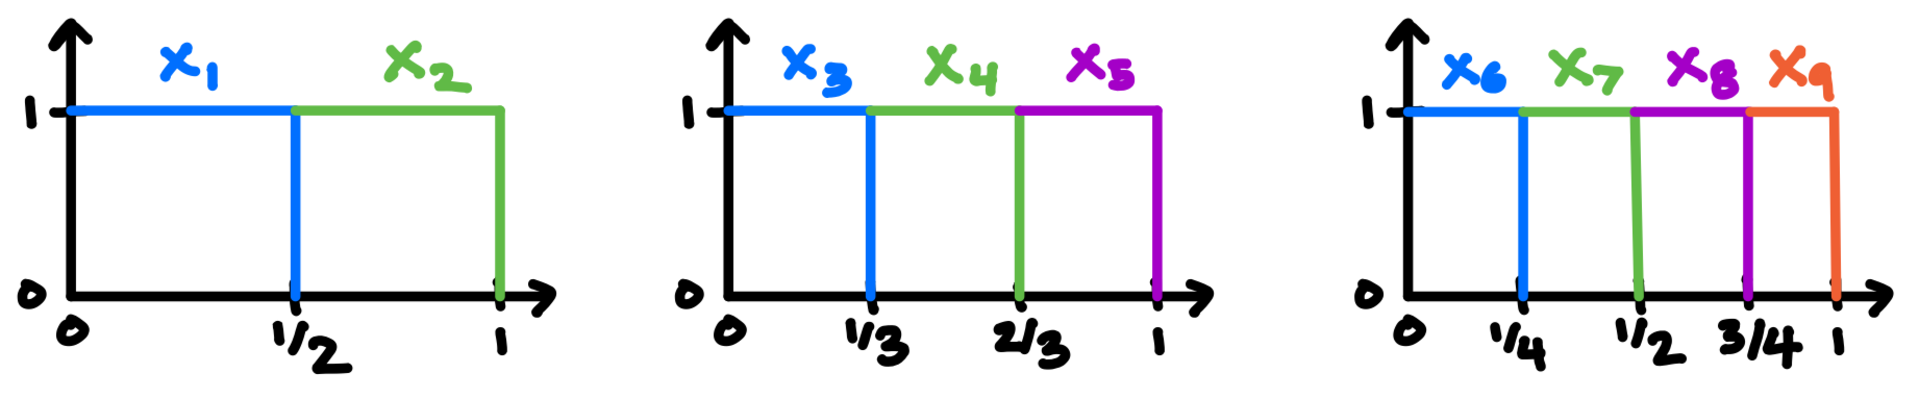
\includegraphics[width = \textwidth]{sliding_box_ex}
	}
	
	This sequence of random variables converges in probability to the zero random variable $X := 0$. This is because for any $\epsilon > 0$ and any $n$, $\mathbb P[|X_n - X| > \epsilon]$ will always be the width of the box, which goes to zero because we've constructed the pulses to decrease their width as soon as we traverse the entire interval. However, $X_n$ \textbf{does not converge} to $X$ almost surely; at each $\omega\in [0, 1]$, no matter how far we go in the sequence, $\omega$ will always be contained in some future box (i.e. given $N\in\mathbb N$, $\exists m > N$ such that $X_m(\omega) = 1$). Thus $X_n(\omega)$ does not converge to $X(\omega)$ at any $\omega\in [0, 1]$, and we don't have almost sure convergence. 
\end{example}

This counterexample shows that convergence in probability does not imply almost sure convergence. Another counterexample with a bit more of a probabilistic flavor goes through using the second Borel-Cantelli lemma as follows. Let $X\equiv 0$ and $X_n\in \{0, 1\}$ be independent with $\mathbb P[X_n = 1] = \frac{1}{n}$. Clearly $X_n\longrightarrow X$ in probability, but $X_n\not\rightarrow X$ almost surely because 
\eq
	\sum_n \mathbb P[|X_n - X| > 0.5] = \sum_n \frac{1}{n} = \infty,
\qe
so the 2nd Borel-Cantelli lemma yields $\mathbb P[|X_n - X| > 0.5\io] = 1$, which shows that $X_n$ converges pointwise to $X$ almost \textit{nowhere}. We'll now prove that the converse is true for finite measures. 

\begin{theorem}
	If $\mu$ is finite, almost sure convergence implies convergence in measure. In particular, almost sure convergence implies convergence in probability.
\end{theorem}
\begin{proof}
	Suppose that $f_n\longrightarrow f$ almost surely and $\mu$ is finite. Since we have a.s. convergence, $\mu(\{ d(f_n, f) > \epsilon\io \}) = 0$, and define
	\eq
		A_n^\epsilon := \bigcup_{m\geq n} \{d(f_m, f) > \epsilon\}.
	\qe
	Note that $A_n^\epsilon\in\mathcal F$ because $\{\omega\in\Omega : d(f_m(\omega), f(\omega)) > \epsilon\}\in\mathcal F$, and $\mu(\limsup A_n^\epsilon) = 0$ because of countable sub-additivity. Thus the reverse Fatou lemma implies that $\limsup \mu(A_n^\epsilon) = 0$. As $A_n^\epsilon\downarrow$ monotonically decreases with $n$, $\limsup \mu(A_n^\epsilon) = \lim\mu(A_n^\epsilon) = 0$, which is equivalent to $f_n\overset{\mu}{\longrightarrow} f$.
\end{proof}

The final theorem of this section is a ``generalization" of the Bolzano-Weierstrauss theorem, which states that every bounded subsequence in $\mathbb R^n$ has a convergent subsequence. 
\begin{theorem}[Convergent subsequences]
	$f_n\longrightarrow f$ in probability iff for every subsequence $(f_{n_m})_m$ of $(f_n)_n$, there exists a convergent subsequence $(f_{n_{m_k}})_k$ of $(f_{n_m})_m$ such that $f_{n_{m_k}}\longrightarrow f$ almost surely as $k\rightarrow\infty$. 
\end{theorem}
\begin{proof}
	We'll use a property of the real numbers: if $(Y_n)_n$ is a sequence in $\mathbb R$ such that $\exists y$ where every subsequence $(Y_{n_k})_k$ has a subsequence $(Y_{n_{m_k}})_k$ such that $Y_{n_{m_k}}\longrightarrow y$ as $k\rightarrow\infty$, then $Y_n\longrightarrow y$. To proceed with the proof, suppose $f_n\longrightarrow f$ in probability and $(f_{n_k})$ is any subsequence. Let $\epsilon_k\downarrow 0$. Since $f_n\longrightarrow f$ in probability, $\exists n_{m_k}$ such that $\forall k\geq n_{m_k}$, we have $\mu(A_k) < 2^{-k}$, where $A_k := \{d(f_n, f) > \epsilon_k\}$. Borel-Cantelli thus implies that $\mu(A_k\io) = 0$, hence $f_{n_{m_k}}\longrightarrow f$ almost surely. For the converse, suppose every subsequence has an almost-surely convergent subsequence, and let $\delta > 0$. Define $Y_n := \mu(\{d(f, f_n) > \delta\})$. The assumptions imply that $Y_n$ has a convergent subsequence, so by the property laid out at the beginning of the proof, we have $Y_n\rightarrow 0$, i.e. we have $f_n\rightarrow f$ in probability. 
\end{proof}

\subsection{Distribution functions}

Distribution functions (a.k.a. cumulative distribution functions) provide a powerful tool to characterize the law of a random variable. The machinery that we've built up so far will allow us to determine the law of the random variable entirely from its distribution function, and many of the statements we make throughout these notes will be written in terms of distribution functions. 

\begin{definition}[Distribution function]
	Let $X$ be a random variable. The \textbf{distribution function} of $X$ is the function $F_X : \mathbb R\rightarrow [0, 1]$ given by
	\eq
		F_X(x) := \mathbb P[X\leq x] = \mathbb P[\{\omega\in\Omega : X(\omega) \in (-\infty, x]\}].
	\qe
\end{definition}

\begin{theorem}
	The distribution function $F_X$ of a random variable $X$ \textbf{uniquely determines} the law $\mathcal L_X$ of $X$. 
\end{theorem}

\begin{proof}
	This is immediate upon noticing that $\{(-\infty, x] : x\in\mathbb R\}$ is a $\pi$-system that generates $\sigB$, so uniqueness follows. 
\end{proof}

As seen in this theorem, the distribution function $F_X$ provides a ``basis" for understanding the law of $X$: it tells us everything we need to know about the law induced by a random variable. It will also provide an easy test to determine if some number of random variables are independent, see for example Theorem~\ref{thm:factor_dist}. We can immediately read off some of the properties of $F_X$.

\begin{theorem}
	$F : \mathbb R\rightarrow [0, 1]$ is a distribution function for a random variable iff the following properties hold:
	\begin{enumerate}[i)]
		\item $F\uparrow$, i.e. $F(x)$ is non-decreasing. 
		\item $\lim_{x\downarrow-\infty} F(x) = 0$ and $\lim_{x\uparrow\infty} F(x) = 1$. 
		\item $F$ is right-continuous, i.e. $\lim_{y\downarrow x} F(y) = F(x)$. 
	\end{enumerate}
\end{theorem}
\begin{proof}
	For the forward direction, suppose $F = F_X$ is the distribution of some random variable $X$. 
	\begin{enumerate}[i)]
		\item If $x\leq y$, then $\{X\leq x\}\subseteq\{X\leq y\}$, so $F_X(x) = \mathbb P[X\leq x] \leq \mathbb P[X\leq y] = F_X(y)$ by monotonicity. 
		\item This is because $(-\infty, x]\downarrow \emptyset$ and $(-\infty, x]\uparrow \Omega$. Continuity from above / below immediately gives the results. 
		\item This is from continuity from above, combined with the fact that $(-\infty, y]\downarrow (-\infty, x]$ as $y\downarrow x$. 
	\end{enumerate}
	For the converse, we need to define a random variable that has this distribution function. Define the random variable on $([0, 1], \sigB|_{[0, 1]}, \Leb|_{[0, 1]})$ given by
	\eq
		X^-(\omega) := \sup\{y\in\mathbb R : F(y) < \omega\}.
	\qe
	The random variable $X^-$ has distribution $F_{X^-} = F$, which you can check by computing $F_{X^-}$. 
\end{proof}

Contrast these properties to those for a Stieltjes measure function, Def.~\ref{def:stieltjes_measure_fn}. The extra property that we have now is (ii): the distribution function must be properly normalized, since we need $\mathbb P[X\leq a]\rightarrow \mathbb P[\Omega] = 1$ as $a\uparrow\infty$. The definition of $X^-$ in the previous proof is called the \textbf{Skorokhod representation} of $F$, and acts as a generalized inverse of a distribution function, since it has the same distribution as $F$. 

\begin{definition}[Skorokhod representation]
	The \textbf{Skorokhod representation} of a random variable $X$ with distribution $F$ is the random variable $X : [0, 1]\rightarrow \mathbb R$ defined by:
	\eq
		X^-(\omega) := \sup\{y\in\mathbb R : F(y) < \omega\}
	\qe
	This satisfies $F_{X^-} = F$. 
\end{definition}

The Skorokhod representation $X^-$ is often denoted by $F^{-1}$, and when $F_X$ is injective and has an inverse $F^{-1}$, $X^- = F^{-1}$, hence the notation. The advantage of the Skorokhod representation is that it exists even when $F_X$ is not injective, and always satisfies the defining property that $F_{X^-} = F$. It also allows one to do some fancy tricks with the uniform distribution.

\begin{theorem}[Probability integral transform]
	Let $X$ be a random variable with a continuous distribution (i.e. $F_X$ is continuous). Then the random variable $U$ defined as
	\eq
		U := F_X(X)
	\qe
	is a uniform random variable on $(\Omega, \mathcal F, \mathbb P)$. 
\end{theorem}
\begin{proof}
	We have
	\eq
		\mathbb P[U\leq x] = \mathbb P[F_X(X)\leq x] = \mathbb P[X\leq F_{X^-}(x)] = F_X(F_{X^-}(x)) = x
	\qe	
	hence $U$ has a uniform distribution.
\end{proof}

A converse statement is that if $U\sim \mathrm{Unif}[0, 1]$ is uniformly distributed on $[0, 1]$, then the random variable
\eq
	F_{X^-}(U)
\qe
has the same law as $X$. If one wants to generate i.i.d. samples from $\mathcal L_X$ on a computer, this is typically the way to go; you can compute $F_{X^-}$, generate uniform samples from $U$, then feed these samples through $F_{X^-}$ to have i.i.d. samples drawn from the law of $X$. This technique is known as \href{https://en.wikipedia.org/wiki/Inverse_transform_sampling}{inverse transform sampling}, and is quite interesting to know. 

\subsection{Independence of random variables}

Next, we consider independence of random variables. Recall that independence is a property of $\sigma$-algebras, or more precisely a property of collections of events. This definition of independence extends naturally to random variables via their generated $\sigma$-algebras. 

\begin{definition}[Independent random variables]
	A collection of random variables $\{X_i\}$ are \textbf{independent} if their generated $\sigma$-algebras, $\{\sigma(X_i)\}$, are independent as $\sigma$-algebras. 
\end{definition}

\begin{definition}[Independent and identically distributed]
	A collection of random variables $\{X_i\}$ are \textbf{independent and identically distributed (i.i.d.)} if $\{\sigma(X_i)\}$ are independent and $\mathcal L_{X_i} = \mathcal L_{X_j}$ for each $i, j$. 
\end{definition}

\begin{example}[Dice rolls (Independence)]
	Intuitively, two random variables $X$ and $Y$ are independent if measuring $X$ gives you no information about the value of $Y$. However, this seems a bit hard to relate to the definition that we've put in place. 
	
	To see the connection, let's do more examples with the six-sided die. Let $X(\omega) := 1$ iff $\omega\in \{a, c, e\}$ and 0 otherwise ($X$ is the indicator telling us if the dice roll was even or odd) and $Y(\omega) := 1$ iff $\omega = f$ and 0 otherwise ($Y$ is the indicator telling us if the dice landed on side $f$). We should expect that $X$ and $Y$ are \textbf{not independent}, because knowing the value of $X(\omega)$ tells us information about what $Y(\omega)$ can be. For example, measuring $X(\omega) = 1$ tells us that the die landed on an even side, which immediately tells us that $Y(\omega) = 0$, since $\omega\neq f$ in this case. To formally show this, note that $\sigma(X)$ and $\sigma(Y)$ are
	\begin{align}
		\sigma(X) = \{ \emptyset, \Omega, \{a, c, e\}, \{b, d, f\}\} && \sigma(Y) = \{ \emptyset, \Omega, \{f\}, \{a, b, c, d, e\}\}.
	\end{align}
	Then $X$ and $Y$ are not independent because for $\{a, c, e\}\in\sigma(X)$ and $\{f\}\in\sigma(Y)$, we have
	\begin{align}
		\mathbb P[\{a, c, e\}\cap \{f\}] = \mathbb P[\emptyset] = 0 && \mathbb P[\{a, c, e\}]\,\mathbb P[\{f\}] = \frac{1}{2}\,\frac{1}{6} = \frac{1}{12},
	\end{align}
	hence we see that $\mathbb P[\{a, c, e\}\cap \{f\}] \neq \mathbb P[\{a, c, e\}]\,\mathbb P[\{f\}]$. 
	
	How do we construct independent random variables? We'll need to consider a second dice roll event, in which the outcome of the second roll does not depend on the outcome of the first roll. That is, we'll use the sample space $\Omega\times\Omega$, whose elements are of the form $(\omega, \omega')$, with $\omega, \omega'\in \Omega$. Let $X$ be the indicator random variable telling us if the \textit{first} roll was even, so $X(\omega, \omega') := 1$ iff $\omega\in \{a, c, e\}$ and 0 otherwise. Likewise, let $Y$ be the indicator of if the \textit{second} roll landed on face $f$, so $Y(\omega, \omega') = 1$ iff $\omega' = f$ and 0 otherwise. Now the situation is:
	\eq
		\sigma(X) &= \{\emptyset, \Omega^2, \{(a, \omega'), (c, \omega'), (e, \omega') : \omega'\in\Omega\}, \{(b, \omega'), (d, \omega'), (f, \omega') : \omega'\in\Omega\} \} \\
		\sigma(Y) &= \{\emptyset, \Omega^2, \{(\omega, f) : \omega\in\Omega\}, \{(\omega, a), (\omega, b), (\omega, c), (\omega, d), (\omega, e) : \omega\in\Omega\} \}.
	\qe
	Unlike the previous example, \textit{these $\sigma$-algebras are independent}. Let's compute the probability of $A\cap B := \{(a, \omega'), (c, \omega'), (e, \omega') : \omega'\in\Omega\} \cap \{(\omega, f) : \omega\in\Omega \}$. Here we have probabilities
	\eq
		\mathbb P[A\cap B] = \mathbb P[\{(a, f), (c, f), (e, f)\}] = \frac{3}{36} = \frac{1}{12} = \frac{1}{2}\times \frac{1}{6} = \mathbb P[A]\,\mathbb P[B]
	\qe
	which is exactly what we want for these events to be independent! We also need to verify the other 3 possible intersections, but these proceed in a very similar manner to show that $X$ and $Y$ are independent. 
\end{example}

% Prop with F factoring iff $X_i$ are independent
We conclude this subsection with a theorem relating independence to the factorization of a joint distribution function. This theorem is very useful to know, as it gives us a concrete corollary of the work we've been doing with independent random variables. 
\begin{theorem}\label{thm:factor_dist}
	Random variables $X_1, ..., X_n$ on $(\Omega, \mathcal F, \mathbb P)$ are \textbf{independent} iff for each $x_1, ..., x_n\in\mathbb R$, 
	\eq
		\mathbb P[X_1\leq x_1, X_n\leq x_n] = \prod_{i = 1}^n \mathbb P[X_i\leq x_i].
	\qe
	In other words, $X_1, ..., X_n$ are independent iff $F_{(X_1, ..., X_n)}(x_1, ..., x_n) = F_{X_1}(x_1)\times ... \times F_{X_n}(x_n)$. 
\end{theorem}
\begin{proof}
	Let $A_i := \{X_i^{-1}((-\infty, b_i] : b_i\in\mathbb R\}$. Then $\sigma(A_i) = \sigma(X_i)$, and $A_i$ are independent $\pi$-systems, which implies that $\sigma(A_i) = \sigma(X_i)$ are independent $\sigma$-algebras. 
\end{proof}

\subsection{Discrete and continuous random variables}
\label{subsec:dist_types}

This section will aim to formalize the notion of a ``discrete" and ``continuous" random variable. Typically when probability is studied rigorously, one does not do much discussion of the difference, instead treating a random variable with a general distribution function for all the theorems. However, more introductory-level probability courses typically separate discrete and continuous distributions, so it's good to have a handle on how to connect all the machinery that we've developed to these definitions. For most of this section, we'll work within the confines of probability measures on $(\mathbb R, \sigB)$; note that all these definitions extend to random variables in the obvious way, since any random variable $X$ induces a probability measure $\mathcal L_X$ on $(\mathbb R, \sigB)$. 

\begin{definition}[Mass]
	We say a probability measure $\mathbb P$ on $(\mathbb R, \sigB)$ \textbf{has mass at $A\in\sigB$} if $\mathbb P[A] > 0$. $\mathbb P$ \textbf{has mass at $x\in\mathbb R$} if $\mathbb P$ has mass at $\{x\}$. A random variable $X$ \textbf{has mass at $A\in\sigB$} if its law $\mathcal L_x$ has mass at $A$. 
\end{definition}

The reason we care about the singleton case is because when $X$ has mass at a singleton, at least part of its distribution is discrete. Equivalently, $X$ has mass at $x$ if $\mathbb P[X = x] > 0$, i.e. if the probability for $X$ to equal a single value is non-zero. Intuitively, this can only happen for discrete distributions, since for a continuous distribution (like $\mathcal N(0, 1)$), only intervals can have non-zero probability. 

% Definition of an atom; problem from pset and proof
\begin{definition}[Non-atomic measure]
	A probability measure $\mathbb P$ on $(\mathbb R, \sigB)$ is \textbf{non-atomic} if for each $A\in\sigB$ with $\mathbb P[A] > 0$, there exists $B\subset A$ strictly such that $B\in\sigB$ and
	\eq
		0 < \mathbb P[B] < \mathbb P[A].
	\qe
	If $\mathbb P$ is not non-atomic, $\mathbb P$ is called \textbf{atomic}. 
\end{definition}

\begin{definition}[Atom]
	Let $\mathbb P$ be an atomic probability measure, and $A\in\sigB$. $A$ is called an \textbf{atom} of $\mathbb P$ if for any $B\subseteq A$ with $B\in\sigB$
	\eq
		\mathbb P[B] \in \{ 0, \mathbb P[A]\}.
	\qe
\end{definition}

\begin{prop}
	Let $\mathbb P$ be a probability measure on $(\mathbb R, \sigB)$, and suppose that $\mathbb P$ gives mass to a singleton $\{x\}\in\sigB$. Then, $\mathbb P$ is atomic, and $\{x\}$ is an atom of $\mathbb P$. 
\end{prop}
\begin{proof}
	This is immediate from the definition: the only subsets of $\{x\}$ are $\emptyset$ and $\{x\}$ itself, both of which have probability in $\{0, \mathbb P[\{x\}]\}$. Thus, $\{x\}$ is an atom and $\mathbb P$ is atomic. 
\end{proof}
Next, we make precise the connection between distribution functions and atoms. Any singleton $\{x\}$ with non-zero mass will induce a discontinuity in $F$ at $x$, as shown in the next theorem. 
\begin{theorem}
	A probability measure $\mathbb P$ is non-atomic iff its distribution function $F(x) := \mathbb P[(-\infty, x]]$ is continuous. 
\end{theorem}
\begin{proof}
	For the forward direction, suppose that $F$ is not continuous. Then $\exists x\in\mathbb R$ and $\epsilon > 0$ such that $\forall\delta > 0$, $F(x) - F(x - \delta) > \epsilon$, since $F$ is not left-continuous at $x$ (note $F$ is always right-continuous) and $F$ is non-decreasing. Now, consider the sequence of sets $A_n := \left(x - \frac{1}{n}, x\right]$. Since $A_n\downarrow \{x\}$, continuity from above implies $\P[A_n]\downarrow \P[\{x\}]$. Since $(-\infty, x] = (-\infty, x - \frac{1}{n}]\sqcup (x - \frac{1}{n}, x]$, we have:
	\begin{equation}
		\P[A_n] = \P\left[(-\infty, x]\right] - \P\left[\left( -\infty, x - \frac{1}{n}\right]\right] = F(x) - F\left(x - \frac{1}{n}\right) > \epsilon
	\end{equation} 
	where the last step follows because $F$ is not left-continuous. This implies that:
	\begin{equation}
		\P[\{x\}] = \lim_{n\rightarrow\infty} \P[A_n]\geq \epsilon > 0,
	\end{equation}
	which shows that $\mathbb P$ is non-atomic, as the singleton set $\{x\}$ has non-zero measure. 
	
	For the converse, suppose that $F(x)$ is continuous, and let $A = (a, b]$ be a finite interval. Suppose that $\P[A] = F(b) - F(a) > 0$. As $F$ is continuous, the intermediate value theorem implies that there exists a point $x_0$ at which $F(x_0) = (F(b) + F(a)) / 2$. Therefore, the measure of $B := (x_0, b]\subseteq A$ is:
	\begin{equation}
		\mathbb P[B] = F(b) - F(x_0) = \frac{F(b) + F(a)}{2} = \frac{1}{2} \mathbb P[A] < \mathbb P[A],
	\end{equation}
	and this is $> 0$ by construction. Note that since $\lim_{x\rightarrow \infty} F(x) = 1$ and $\lim_{x\rightarrow-\infty} F(x) = 0$, the same argument can be made for intervals $(-\infty, a]$ and $(b, \infty)$, so $\mathbb P$ is non-atomic on intervals $\mathcal S$. This also holds for any finite union of intervals $S \in \overline{\mathcal S}$, since if the measure of a finite union of intervals is $> 0$, the measure of at least one of these intervals $I$ must be $> 0$, hence we can apply the previous discussion to $I$. Now, we can extend this property to the entire $\sigma$-algebra $\sigma(\mathcal B_1)$ an \textit{inner measure} and Carath\'eodory. Let $D\in\sigma(\mathcal B_1)$ with $\mathbb P[D] > 0$. As $D$ is measurable, the inner measure from $\mathbb P$ on $\overline{S}$ agrees with the outer measure, hence we may write the measure of $D$ as:
	\begin{equation}
		\mathbb P[D] = \sup_{\cup_i A_i\subseteq D, A_i\in S} \sum_i \mathbb P(A_i) \implies \exists A_i\in S\textnormal{ s.t. } \bigcup_i A_i\subseteq D\textnormal{ and }\mathbb P[D]\geq \sum_i \mathbb P[A_i] \geq \frac{\mathbb P[D]}{2} > 0
	\end{equation}
	by definition of $\sup$. To conclude, there must be at least one $k\in\mathbb Z_+$ such that $\mathbb P[A_k] > 0$, or else $\sum_i \mathbb P[A_i]$ would equal 0. Since $A_k\in S$, we may apply our previous discussions and find $B\subseteq A_k$ with $0 < \mathbb P[B] < \mathbb P[A_k] \leq \mathbb P[D]$, and therefore $D$ cannot be an atom, which completes the proof. Note that the reason we need to use an inner measure is so that $\cup_i A_i\subseteq D$, rather than $D\subseteq \cup_i A_i$. 
\end{proof}

\begin{prop}
	Let $F$ be the distribution function of some random variable. $F$ can have, at most, a countable number of discontinuities. 
\end{prop}
\begin{proof}
	The proof follows from the separability of $\mathbb R$. Let $\mathcal D$ be the discontinuity points of $F$, and suppose that $x\in\mathcal D$. Let $b := F(x)$ and $a := \lim_{y\uparrow x} F(y)$. Then $b > a0$ by definition, and the density of $\mathbb Q\subseteq\mathbb R$ means that $\exists q_x\in\mathbb Q$ such that $b > q_x > a$. This generates an injection $\mathcal D\hookrightarrow \mathbb Q$, $x\mapsto q_x$, hence $|\mathcal D|$ must be at most $|\mathbb Q|$. 
\end{proof}

We are now in a position to define a continuous and discrete random variable in terms of the properties of its distribution function. Not every random variable will be discrete or continuous; there are also ``mixed" random variables that have distributions that are continuous in one domain, but discrete in the other. The advantage of the formalism we've developed is that we don't care whether a random variable is discrete, continuous, or mixed; all of them are on the same footing. 

\begin{definition}[Continuous random variable]
	A random variable $X$ is continuous iff $F_X$ is continuous.
\end{definition}

\begin{corollary}
	A random variable $X$ is continuous iff it is non-atomic. 
\end{corollary}

\begin{definition}[Discrete random variable]
	A random variable $X$ is \textbf{discrete} if its image $X(\Omega)$ is countable. 
\end{definition}

\begin{corollary}
	Any discrete random variable $X$ is atomic.
\end{corollary}
Note that unlike the continuous case, this is \textit{not an iff statement}; the converse is not true in general. This is because $X$ can be atomic but have a mixed distribution, it need not have a discrete distribution. 

Atoms play a very intuitive role in the theory of discrete probability measures: any set with non-zero measure is simply a union of some (countable) number of atoms. Suppose $X$ is a discrete random variable with image $X(\Omega) = \{x_i \in\mathbb R : i\in\mathbb N\}$. Each $\{x_i\}$ with non-zero mass is an atom of $X$, and we will denote the set of atoms with $\{a_j\}$. The law of $X$ is completely characterized by the probabilities, as for each $A\in\sigB$
\begin{align}
	p_i := \mathbb P[X = x_i] && \mathcal L_X[A] = \sum_{x_i\in A} p_i = \sum_{a_j\in A} p_j
\end{align}
because of countable additivity\footnote{Here the first sum is over all values in the image, while the second sum is over all atoms. These will always yield the same result because if $x_i$ is not an atom, then $p_i = 0$.}. We can also describe the amount of information contained by the random variable $X$ via its $\sigma$-algebra $\sigma(X)$, which is simply the pull-back of each $\{x_i\}$:
\eq
	\sigma(X) = \left\{ \{X = x_i\} : i\in\mathbb N \right\}
	\label{eq:discrete_rv_sigma_X}
\qe
This should make sense, because the information given to us by $X$ is just the distinct values $x_i$ it takes on. Note that although the values in the image that are not atoms, $z\in \{x_i\}\setminus \{a_j\}$, have no probability, they are still included in $\sigma(X)$. However, they will not influence any probabilistic statements, since $\mathbb P[X = z] = 0$. 

\begin{example}[Independence of discrete random variables]
	If you've taken a probability class before, you've probably seen independence phrased in the following way. Two discrete random variables $X$, $Y$ are independent if
	\eq
		\mathbb P[X = x, Y = y] = \mathbb P[X = x]\,\mathbb P[Y = y]
		\label{eq:indep_finite}
	\qe
	for each $x\in X(\Omega)$, $y\in Y(\Omega)$. Since we know the structure of $\sigma(X)$ and $\sigma(Y)$ from Eq.~\eqref{eq:discrete_rv_sigma_X}, we now immediately derive Eq.~\eqref{eq:indep_finite}. For each $x\in X(\Omega), y\in Y(\Omega)$, independence tells us that the sets $\{X = x\}\in\sigma(X)$ and $\{Y = y\}\in\sigma(Y)$ are independent, which implies
	\eq
		\mathbb P[X = x, Y = y] = \mathbb P[\{X = x\}\cap \{Y = y\}] = \mathbb P[X = x]\,\mathbb P[Y = y].
	\qe
\end{example}

\subsection{Tail $\sigma$-algebras}

We often wish to determine the information afforded to us by an infinite sequence of random variables $(X_i)$. 

{\color{red}TODO}

% include stackexchange post
% Include infinite coin flip example

\newpage
\section{Integration and Expectation}

Measure spaces allow us to generalize the notion of (unsigned\footnote{Here is a \href{https://math.stackexchange.com/questions/49641/integration-of-forms-and-integration-on-a-measure-space?rq=1}{great discussion} on the broad types of integration.}) integration to other spaces that are more abstract than Euclidean space. Any measure space admits the notion of integration, as we'll soon see. The idea is to define the integral on piecewise-constant (simple) functions, where the integral should intuitively be the function value on each constant set, times the measure of the set. The machinery we've built up with convergence of measurable maps then allows us to approximate \textit{any integrable function} with simple functions, leading to a chain of integral definitions for different classes of functions
\eq
	\textnormal{simple} \longrightarrow \textnormal{bounded + finite support} \longrightarrow \textnormal{non-negative} \longrightarrow \textnormal{integrable}
	\label{eq:steps_of_integral_construction}
\qe
that are all built on top of one another. This section will define what all these types of functions look like, and how we explicitly build up the integral to each new class of function. 

For this section (and really the remainder of these notes), we'll be working with measurable maps $f : (\Omega, \mathcal F)\rightarrow (\mathbb R, \sigB)$, under the assumption that the measure space $(\Omega, \mathcal F, \mu)$ \textbf{is $\sigma$-finite}. You can see in some of the theorems why we need this: allowing our space to be covered by sets of finite measure will be very useful in our discussion of integration. One can generalize the integral to measurable maps $(\Omega, \mathcal F)\rightarrow (E, \mathcal E)$, where $E$ is a Banach space and $\mathcal E$ is the associated Borel $\sigma$-algebra, but for our intents and purposes we'll almost always be working with random variables, so we don't need to do this. If you're interested in this construction, feel free to check out my notes on measure theory. 

\subsection{Simple functions}

Simple functions are the most basic types of functions we can integrate. We'll define the integral of a simple function in an intuitive manner, then show that we can approximate bounded functions with simple functions. Let's start with some definitions.

\begin{definition}[Indicator function]
	For $A\in\mathcal F$, the \textbf{indicator function on $A$} is the measurable map $1_A : (\Omega, \mathcal F)\rightarrow (\mathbb R, \sigB)$,
	\eq
		1_A(\omega) := \begin{cases}1 & \omega\in A \\ 0 & \omega\notin A \end{cases}. 
	\qe
\end{definition}
\begin{definition}[Simple function]
	A \textbf{simple function} is any function $f : \Omega\rightarrow\mathbb R$ of the form 
	\eq
		f(\omega) = \sum_{i = 1}^n a_i 1_{A_i}(\omega)
	\qe
	for $a_1, ..., a_n\in\mathbb R$ and $A_1, ..., A_n\in\mathcal F$ are disjoint. 
\end{definition}

In other words, a simple function $f = \sum_{i = 1}^n a_i 1_{A_i}$ is a piecewise-constant function that only takes on a finite number of values. We'll also occasionally use notation like $1_{x\leq a}$ or $1_{X\in A}$, for indicator functions on $\mathbb R$ and $\Omega$ respectively, given by $1_{(-\infty, a]}$ and $1_{\{X\in A\}}$. 

% Include monotone class lemma here.
\begin{lemma}[Simple approximation]
	Let $X : (\Omega, \mathcal F)\rightarrow (\mathbb R, \sigB)$ be a random variable. Then, there exists a set of simple functions $f_n : (\Omega, \mathcal F)\rightarrow (\mathbb R, \sigB)$ such that $f_n(\omega)\uparrow f(\omega)$ at each $\omega\in\Omega$. 
\end{lemma}
\begin{proof}
	Define $\eta_n : \mathbb R\rightarrow R$ by 
	\eq
		\eta_n(x) := n 1_{x\geq n} + \sum_{k = 0}^{2^n - 1} k 2^{-n} 1(x).
	\qe
	This map essentially ``chops up" the function into a simple function, and is always increasing by construction (I would recommend drawing a picture of it). Suppose $f\geq 0$ (if $f$ is not $\geq 0$, decompose $f = f_+ + f_-$, where each part is non-negative; we'll do this extensively soon), and set $f_n := \eta_n(f)$. Then $f_n$ is a simple function, and $f\geq f_{n + 1}\geq f_n$ for each $n$ with $f(\omega) - f_n(\omega)| < 2^{-n}$ by construction. This implies $f_n(\omega)\uparrow f(\omega)$ at each $\omega\in\Omega$, and completes the proof of the lemma. 
\end{proof}

Before moving to integration, we make a brief digression into the monotone class theorem. This theorem is important for characterizing classes of functions; it's a bit formal, but will prove essential to some of the proofs we will do later on in these notes. There are actually two versions of this theorem: one for bounded functions, and one for arbitrary measurable functions. 

\begin{theorem}[Monotone class theorem]
	Let $\mathcal H$ be a collection of functions $\Omega\rightarrow\mathbb R$ such that
	\begin{enumerate}[i)]
		\item The constant function $1\in\mathcal H$. 
		\item $\mathcal H$ is a vector space over $\mathbb R$. 
		\item If $h_n\in\mathcal H$ is a sequence of non-negative functions such that $h_n\uparrow h$ with $h : \Omega\rightarrow\mathbb R$ (is a bounded function), then $h\in\mathcal H$. 
	\end{enumerate}
	Under these assumptions, if $\rho$ is a $\pi$-system and $1_A\in\mathcal H$ for each $A\in\rho$, then $H$ contains all (bounded) $\sigma(\rho)$-measurable functions. 
\end{theorem}
\begin{proof}
	It suffices to show that $1_S\in\mathcal H$ for any $S\in\sigma(\rho)$ by the simple approximation lemma. To, let $\mathcal L := \{A\subseteq\Omega : 1_A\in\mathcal H\}$. The assumptions tell us that $\mathcal L$ is a $\lambda$-system:
	\begin{enumerate}[i)]
		\item $\Omega\in\mathcal L$ since $1\in\mathcal H$. 
		\item Let $A, B\in\mathcal L$ with $A\subseteq B$. Then $1_A, 1_B\in\mathcal H$, and in particular $1_{B\setminus A} = 1_B - 1_A\in\mathcal H$ because it is a vector space, so $B\setminus A\in\mathcal L$. 
		\item If $A_n\in\mathcal L$ with $A_n\uparrow A$, then $1_{A_n}\uparrow 1_A$ implies $1_A\in\mathcal H$, thus $A\in\mathcal L$. 
	\end{enumerate}
	This verifies that $\mathcal L$ is a $\lambda$-system, and Dynkin's $\pi$-$\lambda$ theorem immediately gives that $\sigma(\rho)\subseteq\mathcal L$, hence we see that $\mathcal H$ contains all indicator functions on $\sigma(\rho)$ as desired. 
\end{proof}

\subsection{Construction of the integral}

With our discussion of simple functions complete, we now move on to the main topic of this section: \textbf{constructing the integral}. We begin by integrating simple functions, since their form provides an intuitive definition. They are piecewise constant, so we just need to define the integral to be exactly what we expect it to be: the value of the function on each constant slice, times the measure of that slice. 
\begin{definition}[Integral of a simple function]
	Let $f := \sum_{i = 1}^n a_i 1_{A_i}$ be a simple function. We define the \textbf{integral} of $f$ to be
	\eq
		\int f\,d\mu := \sum_{i = 1}^n a_i\, \mu(A_i).
	\qe
\end{definition}

Before moving on, we state some useful properties of the integral. These properties are quite basic and they will turn out to hold at \textbf{each stage in our construction}, so this theorem is actually four theorems, packaged together neatly. 
\begin{theorem}[Properties of $\int f\,d\mu$]
	Let $f$ and $g$ be simple (bounded + finite support) ((non-negative)) (((integrable))) functions.
	\begin{enumerate}[i)]
		\item If $f\geq 0$ a.s., then $\int f\,d\mu\geq 0$. 
		\item (Linearity I) For $a\in\mathbb R$, $\int af\,d\mu = a\int f\,d\mu$. 
		\item (Linearity II) $\int (f + g)\,d\mu = \int f\,d\mu + \int g\,d\mu$. 
		\item (Monotonicity) If $f\geq g$ a.s., then $\int f\,d\mu\geq \int g\,d\mu$. 
		\item (Equality) If $f = g$ a.s., then $\int f\,d\mu = \int g\,d\mu$. 
		\item (Absolute value) We have
		\eq
			\left| \int f\,d\mu \right| \leq \int |f|\,d\mu.
		\qe
	\end{enumerate}
\end{theorem}
We'll also frequently be using the notation
\eq
	\int_A f\,d\mu := \int f 1_A\,d\mu
\qe
which holds for any $f$ that we've defined the integral of. 

The next step in Eq.~\eqref{eq:steps_of_integral_construction} is to extend the definition of the integral from simple functions to \textbf{bounded functions with finite support}. Before doing this, we should be precise about what a bounded function with finite support is. We will extend the definition of an integral by approximating such a function with simple functions.
\begin{definition}[Bounded, finite support]
	A function $f$ is \textbf{bounded} if $\exists M > 0$ such that $|f| \leq M$. The function $f$ has \textbf{finite support} if $\exists S\in\mathcal F$ such that $\mu(S) < \infty$ and $f(\omega) = 0$ for each $\omega\in S^c$. 
\end{definition}

\begin{definition}[Integral of a bounded function with finite support]
	Suppose that $f$ is bounded with finite support. We define its integral to be
	\eq
		\int f\,d\mu := \sup_{\alpha\textnormal{ simple, }\alpha\leq f,\; \alpha|_{S^c}\equiv 0} \int \alpha\,d\mu = \inf_{\beta\textnormal{ simple, }f\leq \beta,\; \beta|_{S^c}\equiv 0} \int \alpha\,d\mu
	\qe
\end{definition}

In this definition, we've approximated $f$ from below with simple functions $\alpha$ and take the supremum of these integrals, and approximated $f$ from above with simple functions $\beta$, taking the infimum of these integrals. We need to show that these two definitions agree, i.e. that $\int f\,d\mu$ is well-defined. That $\sup \int \alpha\,d\mu \leq \inf \int \beta\,d\mu$ is immediate, since $\alpha\leq f\leq \beta$ by construction, but it remains to show the other direction. Let $M$ be an upper bound for $f$ with support $S$, and define simple functions $\alpha_n$ and $\beta_n$ as
\begin{align}
	A_k := \left\{\frac{M(k - 1)}{n} < f < \frac{kM}{n} \right\} && \alpha_n := \sum_{k =-n}^n \frac{(k - 1)M}{n} 1_{A_k} && \beta_n := \sum_{k =-n}^n \frac{kM}{n} 1_{A_k}.
\end{align}
Since $\bigcup_{k = -n}^n A_k= S$, as $\beta_n - \alpha_n = \frac{M}{n} 1_{S}$ we have $\int (\beta_n - \alpha_n)\,d\mu = \frac{M}{n} \mu(S)$, which in particular is finite and goes to zero as $n\rightarrow\infty$. We thus have (using linearity of the integral of simple functions):
\eq
	\sup_\alpha\int\alpha\,d\mu\geq \int\alpha_n\,d\mu = \int\beta_n\,d\mu - \frac{M}{n}\mu(S) \geq \inf_\beta\int\beta\,d\mu - \frac{M}{n}\mu(S) \uparrow \inf_\beta\int\beta\,d\mu,
\qe
where taking $n\uparrow\infty$ gives the desired result to show that $\int f\,d\mu$ is well-defined. 

The third step of Eq.~\eqref{eq:steps_of_integral_construction} is to extend the definition of $\int f\,d\mu$ from bounded + finite support functions to \textbf{non-negative functions}. This step of the process is very similar to the previous one, only now we approximate an arbitrary non-negative function with a sequence of functions that are bounded with finite support. 
\begin{definition}[Integral of a non-negative function]
	Let $f$ be a non-negative function. The \textbf{integral} of $f$ is defined as
	\eq
		\int f\,d\mu := \sup\left\{ \int h\,d\mu : 0\leq h \leq f, \textnormal{ $h$ bounded, } \mu(h > 0) < \infty \right\}.
	\qe
\end{definition}

\begin{lemma}
	Let $f\geq 0$, $A_n\in\mathcal F$ with $\mu(A_n) < \infty$ and $A_n\uparrow\Omega$. Then
	\eq
		\int_{A_n} (f\wedge n)\,d\mu \uparrow \int f\,d\mu
	\qe
	as $n\rightarrow\infty$, where recall $x\wedge n := \min\{x, n\}$. 
\end{lemma}
Since we're working with a $\sigma$-finite measure space, we can always find such a sequence of $A_n\in\mathcal F$ as required by the lemma. 

The final step is to extend this construction to \textbf{integrable functions}. We first define what we mean by integrable.
\begin{definition}[Integrable function, integral of an integrable function]
	A measurable map $f$ is \textbf{integrable} if 
	\eq
		\int |f|\,d\mu < \infty.
	\qe
	Decompose $f$ as
	\begin{align}
		f := f^+ - f^- && f^+ := \max\{f, 0\} = f\vee 0 && f^- := \max\{-f, 0\} = (-f)\vee 0.
	\end{align}
	The \textbf{integral} of an integrable function $f$ is
	\eq
		\int f\,d\mu := \int f^+\,d\mu - \int f^-\,d\mu.
	\qe
\end{definition}
Note both $f^+, f^-\geq 0$, so this definition is valid. This completes the construction of the integral! Let's discuss a few specific cases. 
\begin{itemize}
	\item When we are working with the Lebesgue measure on $\mathbb R^n$ and an integrable function $f : \mathbb R^n\rightarrow\mathbb R$, we write
	\eq
		\int f(x)\, d^nx := \int f(x)\,d\Leb (x).
	\qe
	\item The integral of a random vector $X = (X_1, ..., X_n)$ on $\mathbb R^n$ is just the integral of each component,
	\eq
		\int X\,d\mathbb P := \left( \int X_1\,d\mathbb P, ..., \int X_n\,d\mathbb P \right).
	\qe
	\item The \textbf{Stieltjes integral} is the integral of a function $f(x)$ with respect to the measure $\mu$ corresponding to Stieltjes function $G(x)$, i.e. $\mu((a, b]) := G(b) - G(a)$. This is written
	\eq
		\int f\,d\mu = \int f(x)\,dG(x).
	\qe
	\item When working with a countable sample space, $\mathcal F := 2^\Omega$, and $\mu$ the counting measure on $\Omega$, the integral reduces down to a sum:
	\eq
		\int f\,d\mu = \sum_{\omega\in\Omega} f(\omega).
	\qe
\end{itemize}

%\subsection{Basic properties of integration}

\subsection{$L^q$ spaces}

% Construction of the L^q Banach space (mod out by functions that are a.e. zero)

Now that we've defined the integral, given a measurable space, we can investigate an associated class of function spaces called the $L^q$ spaces. This construction will work for an arbitrary $\sigma$-finite measure space, but we'll focus on probability measures here; most of the work we do will follow through immediately if $(\Omega, \mathcal F, \mu)$ is $\sigma$-finite rather than a probability measure. 

\begin{definition}[$q$-norm, $L^q$ space]
	Let $f : (\Omega, \mathcal F, \mu)\rightarrow \mathbb R$ be measurable. The \textbf{$q$-norm} of $f$ is
	\eq
		||f||_q := \left( \int |f|^q\,d\mu \right)^{\frac{1}{q}}.
	\qe
	We let $L^q(\mu)$ denote the space of $q$-integrable functions, 
	\eq
		L^q(\mu) := \left\{ f : (\Omega, \mathcal F, \mu)\rightarrow \mathbb R : ||f||_q < \infty \right\} 
	\qe
\end{definition}

\subsection{Expectation and inequalities}

\subsection{Convergence theorems}

\section{Weak convergence}

\subsection{Relation with other modes of convergence}

%\section{Convergence}
%\subsection{Almost-surely, in probability, in $L^q$}
%\subsection{Convergence theorems}
%\subsection{Weak convergence}

% include relations between convergence, maybe draw out a map

\section{Product Spaces}

\section{Conditional Expectation}

\section{Laws of large numbers}

\section{Characteristic Functions and the Central Limit Theorem}

\subsection{Characteristic functions}

\subsection{The Central Limit Theorem}

\subsection{Related topics}
% Poisson approximation
% Lindenberg method
% Law of iterated logarithms

% If time
%\section{Concentration of measure}
%\section{Large deviations}

% May want to make another set of notes on stochastic processes

\section{Martingales}

\section{Markov chains}

\end{document}